\documentclass{report}

\usepackage{graphicx}
\usepackage{amsmath}
\usepackage{float}

\title{\textbf{ML + CSP} \\ Movie Recommender System}
\author{Rabottini Simone \\ Calcaterra Giacomo}
\date{21 Febbraio 2023}

\begin{document}

\maketitle

\begin{abstract}
    Viene descritto lo sviluppo di un recommender system di film realizzato in Python attraverso l'uso del Machine Learning e del Constraint Satisfaction Problem (CSP). \\
    Il sistema, implementato in un'applicazione web, utilizza un approccio di filtraggio basato sul contenuto, analizzando le caratteristiche dei film, come il genere e il regista, per effettuare raccomandazioni personalizzate agli utenti; i risultati inoltre, possono essere filtrati tramite la risoluzione di un problema CSP. I dati utilizzati provengono dal dataset di "The Movie Database" (TMDb), che contiene metadati sui film e valutazioni di film da parte degli utenti. \\ 
    Questo report mette in mostra l'efficacia del filtraggio basato sul contenuto nell'ambito dei recommender system di film ed esplora le caratteristiche del sistema.
\end{abstract}

\tableofcontents

\newpage
\chapter{Introduzione}
    Per il progetto di "Fondamenti e Applicazioni dell'Intelligenza Artificiale" è stato scelto di realizzare un Recommender System di film attraverso l'uso del Machine Learning e del Constraint Satisfaction Problem (CSP). \\
    L'obiettivo è quello di realizzare un sistema che utilizza il Machine Learning per raccomandare nuovi film che potrebbero piacere all'utente in base a un film dato in input. Il sistema utilizza un tipo di apprendimento non supervisionato chiamato “filtraggio basato sul contenuto”, che si basa sulla descrizione e sui metadati del film, per effettuare raccomandazioni. \\
    Inoltre, i risultati da restituire all'utente possono essere filtrati  attraverso la risoluzione di un problema CSP con constraints. Dalle raccomandazioni effettuate dal ML ottieniamo le variabili del problema (i nomi dei film), e i constraints vengono applicati al problema in base a filtri scelti dall'utente, che nel nostro caso possono essere genere, anno di uscita, e/o durata del film. \\
    I recommender system sono strumenti di filtraggio delle informazioni che vengono utilizzati per prevedere le preferenze degli utenti e suggerire prodotti, film e altro. Il loro impiego è fondamentale al fine di guidare gli utenti in diversi contesti, come nella scelta di film nel nostro caso oppure nello shopping online. La loro importanza è data dal loro ampio utilizzo in diverse applicazioni come Amazon, Netflix, Spotify e diverse altre, al fine di migliorare l'esperienza dell'utente e aumentare la fidelizzazione del cliente. Di seguito verranno mostrati alcuni esempi:
    
    %screen Spotify
    \begin{figure}[h]
            \centering
            
\includegraphics[width=1\linewidth]{screenshot/spotify_example.png}
            \caption{Sistema di raccomandazione di Spotify}
            \label{fig:enter-label}
        \end{figure}
    %screen Netflix
    \begin{figure}[h]
            \centering
            
\includegraphics[width=1\linewidth]{screenshot/netflix_example.png}
            \caption{Sistema di raccomandazione di Netflix}
            \label{fig:enter-label}
        \end{figure}

\newpage
\chapter{Materiali e Metodi}
    \section{Dataset}
        I dati utilizzati dal sistema provengono dal dataset di "The Movie Database" trovato su Kaggle.com, piattaforma di data science. Quest'ultimo offre due dataset che forniscono metadati su circa 4800 film usciti dal 1916 al 2017: \\
        "movies" contiene informazioni sui film come id, titolo, generi, budget, incassi ecc. \\
        "credits" contiene informazioni sui film riguardo i partecipanti quali attori, regista e crew. Al fine di visualizzare e utilizzare questi dati in mode agevole, i due dataset vengono uniti, estrapolando esclusivamente le colonne utili allo scopo del sistema:
        \begin{figure}[h]
            \centering
            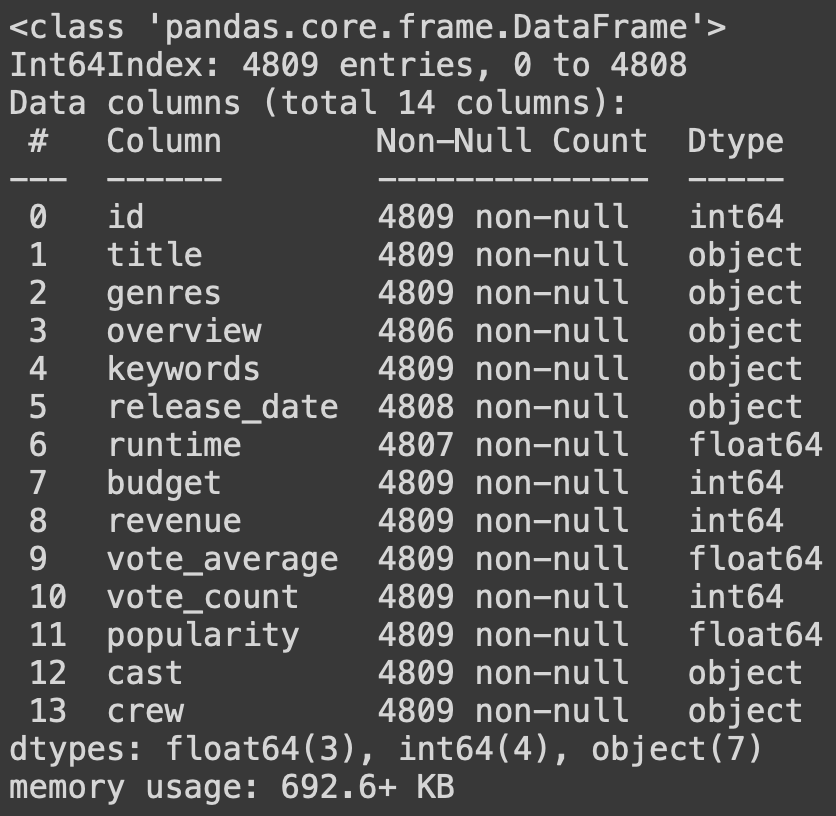
\includegraphics[width=0.5\linewidth]{screenshot/movies.info().png}
            \caption{Features finali}
            \label{fig:enter-label}
        \end{figure}
        
        \begin{itemize}
            \item \textbf{id}: identificativo del film nel database di TMDb
            \item \textbf{title}: titolo del film
            \item \textbf{genres}: generi associati al film
            \item \textbf{overview}: trama del film
            \item \textbf{keywords}: parole chiavi e tags del film
            \item \textbf{release\_date}: data di uscita del film
            \item \textbf{runtime}: durata del film
            \item \textbf{budget}: budget stanziato per la realizzazione del film
            \item \textbf{revenue}: incassi totali ottenuti dal film 
            \item \textbf{vote\_average}: votazione media ottenuta dal film da parte degli utenti di TMDb
            \item \textbf{vote\_count}: numero di voti ricevuti dal film da parte degli utenti di TMDb
            \item \textbf{popularity}: indice di popolarità, misura che riflette quanto un film sia conosciuto o discusso dagli utenti. 
            \item \textbf{cast}: attori che hanno partecipato alla realizzazione del film
            \item \textbf{crew}: troupe che ha realizzato il film (regista, sceneggiatore...) 
        \end{itemize}
        \begin{figure}[h]
            \centering
            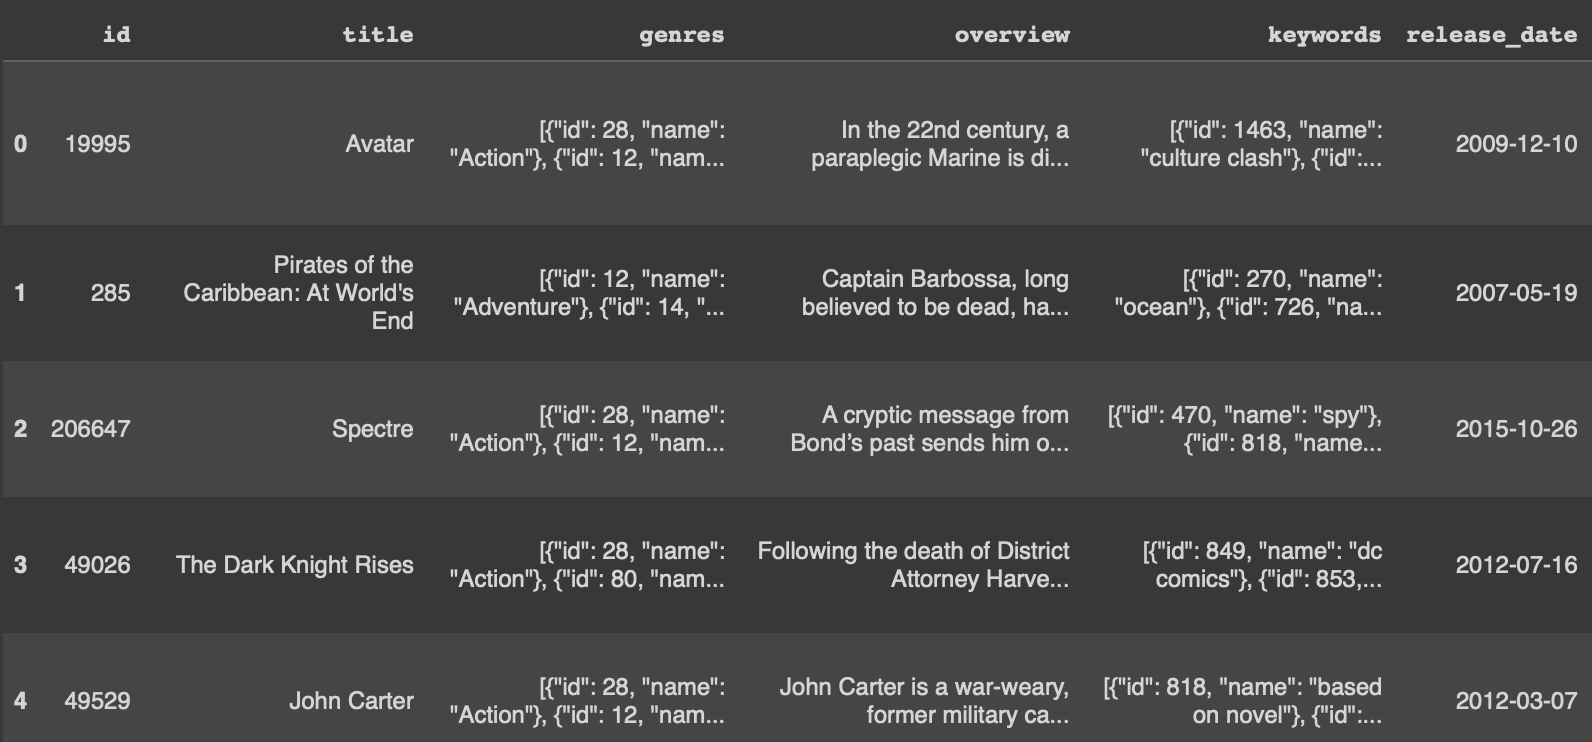
\includegraphics[width=1\linewidth]{screenshot/movies.head1.png}
            \caption{(1/2) Head del dataframe finale}
            \label{fig:enter-label}
        \end{figure}
        \begin{figure}[h]
            \centering
            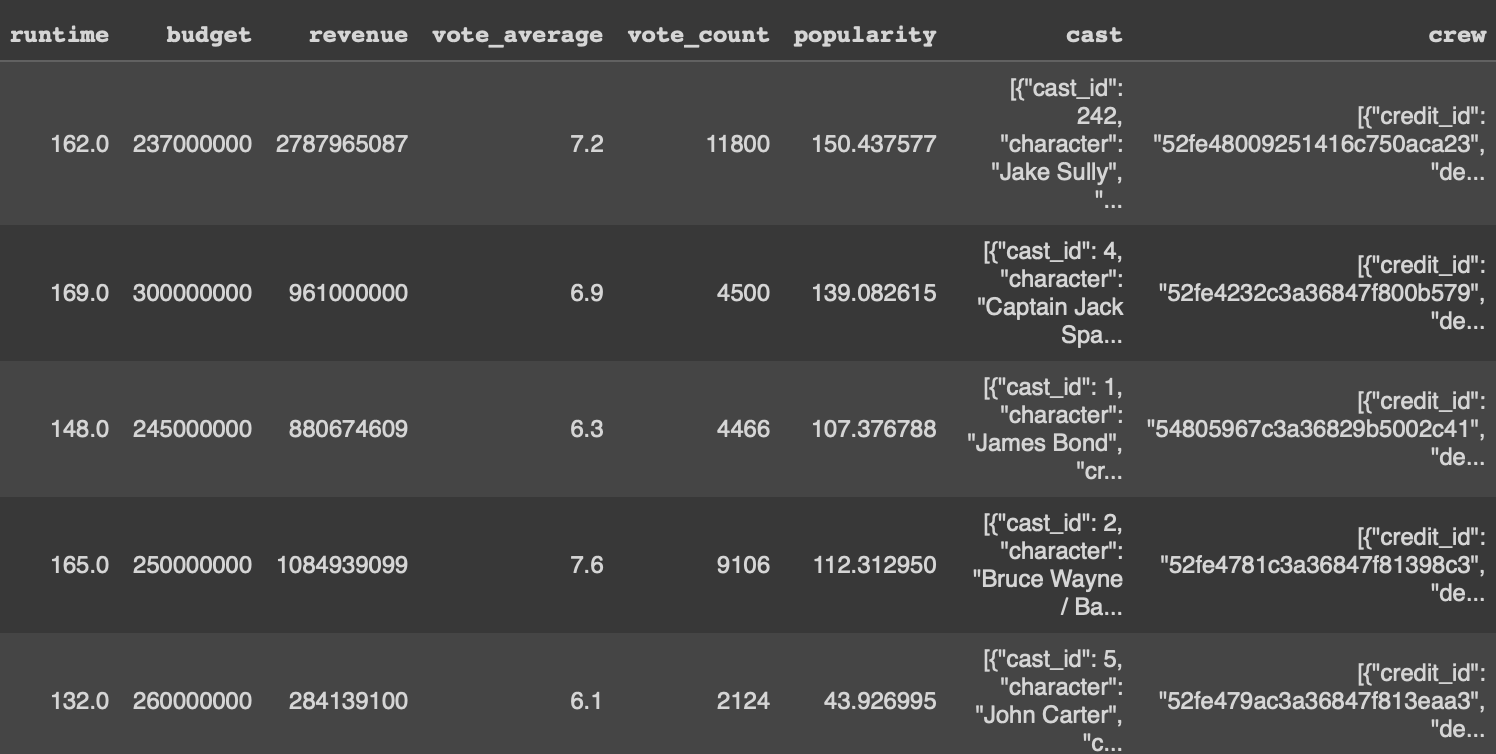
\includegraphics[width=1\linewidth]{screenshot/movies.head2.png}
            \caption{(2/2) Head del dataframe finale}
            \label{fig:enter-label}
        \end{figure}
        
    \section{Librerie}
        Sono state utilizzate diverse librerie Python, ognuna per uno scopo ben preciso. \\
        \begin{itemize}
            \item \textbf{Pandas}: manipolazione, gestione e visualizzazione di dataframe
            \item \textbf{Abstract Syntax Tree (ast)}: utilizzato nel nostro caso nella fase di Data cleaning e preparation per valutare le liste di dizionari (ad esempio dei generi) e trasformarle in liste. Questo va a facilitare la loro analisi e manipolazione
            \item \textbf{scikit-learn}: utilizzata per sviluppare il core del nostro Machine Learning:
            \begin{itemize}
                \item \textbf{CountVectorizer}: feature extraction e addestramento del modello
                \item \textbf{cosine\_similarity}: metrica che stabilisce la somiglianza tra contenuti (nel nostro caso tra vettori ottenuti dal passo precedente) calcolata come il coseno dell'angolo tra di essi
            \end{itemize}
            \item \textbf{Natural Language Toolkit (NTLK)}: libreria di elaborazione del linguaggio naturale che nel nostro caso, attraverso l'algoritmo di Stemming di Porter (PorterStemmer), rimuove i suffissi comuni delle parole riducendole alla radice. Ciò viene fatto per ridurre la dimensione del vocabolario e facilitare il processo di riconoscimento di parole diverse ma correlate
            \item \textbf{Python-constraint}: gestione, manipolazione e risoluzioni dei problemi CSP, che nel nostro caso hanno un ruolo di filtraggio dei risultati da restituire all'utente finale
            \item \textbf{streamlit}: utilizzata per costruire l'interfaccia grafica del sistema. Questa libreria facilita lo sviluppo e il deploy di applicazioni web ed è mirata per l'utilizzo del Machine Learning
            \item \textbf{request}: utilizzata dall'applicazione web per effettuare richieste HTTP. Nel nostro caso la utilizziamo per interagire con l'API di TMDb per ottenere i poster dei film da restituire insieme ai risultati nel sistema
        \end{itemize}

    \section{Data cleaning e preparazione}
        Prima di realizzare la funzione di raccomandazione è stato preparato il dataframe al fine di incentivare il funzionamento e incrementare le performance del sistema. \\ Dopo aver constatato di avere diverse colonne con valori null, è stato deciso di rimuovere queste entries insieme ai duplicati, che potrebbero compromettere in particolare il funzionamento del Constraint Satisfaction Problem. \\
        Diverse colonne risultano difficili da interpretare o inutilizzabili per gli scopi del sistema, pertanto vanno trasformate:
        \begin{figure}[h]
            \centering
            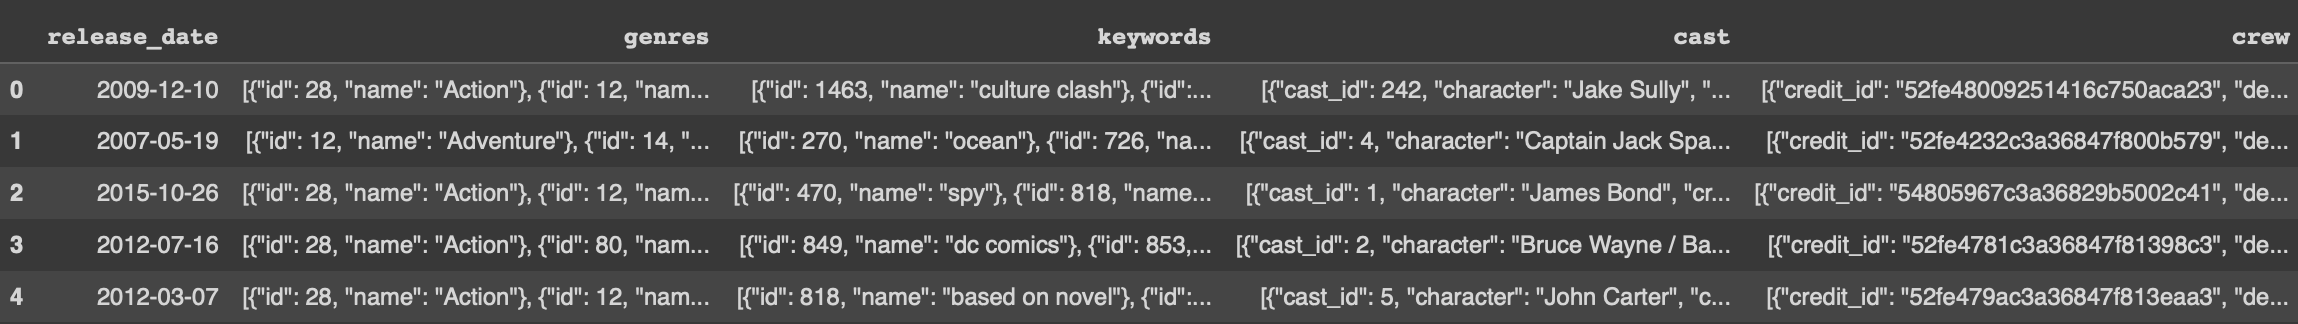
\includegraphics[width=1\linewidth]{screenshot/convert_features.png}
        \end{figure}
        \begin{itemize}
            \item \textbf{release\_date}: da tipo "object" è stato dapprima trasformato in "datetime", per poi estrarne esclusivamente la data in tipo intero. Ciò è stato svolto in quanto la Data di Uscita di un film è un filtro applicabile, e il tipo int facilita sicuramente i controlli (es. release\_date $>=$ 2014)
            \item \textbf{genres, keywords, cast, crew}: attraverso delle funzioni scritte ad-hoc per effettuare la conversione; vengono valutate le liste di dizionari, si ottiene esclusivamente il campo del nome e si aggiunge di volta in volta in una lista. Prendendo ad esempio il genere, così facendo otteniamo una lista di generi associati (con solo i nomi) partendo da che una lista di dizionari (dove per ognuno c'è campo id e campo titolo). Nel caso del cast e della crew vengono estratti esclusivamente i più significativi, rispettivamente i primi 3 attori e il regista.
        \end{itemize}
        Infine, per favorire il lavoro del Machine Learning, si eliminano eventuali spazi. Viene trasformato quindi anche il campo "Overview" da stringa in lista di stringhe senza spazi. \\
        Tutto ciò che è stato appena realizzato va a facilitare la analisi e manipolazione dei dati. Di seguito il risultato finale:
        \begin{figure}[h]
            \centering
            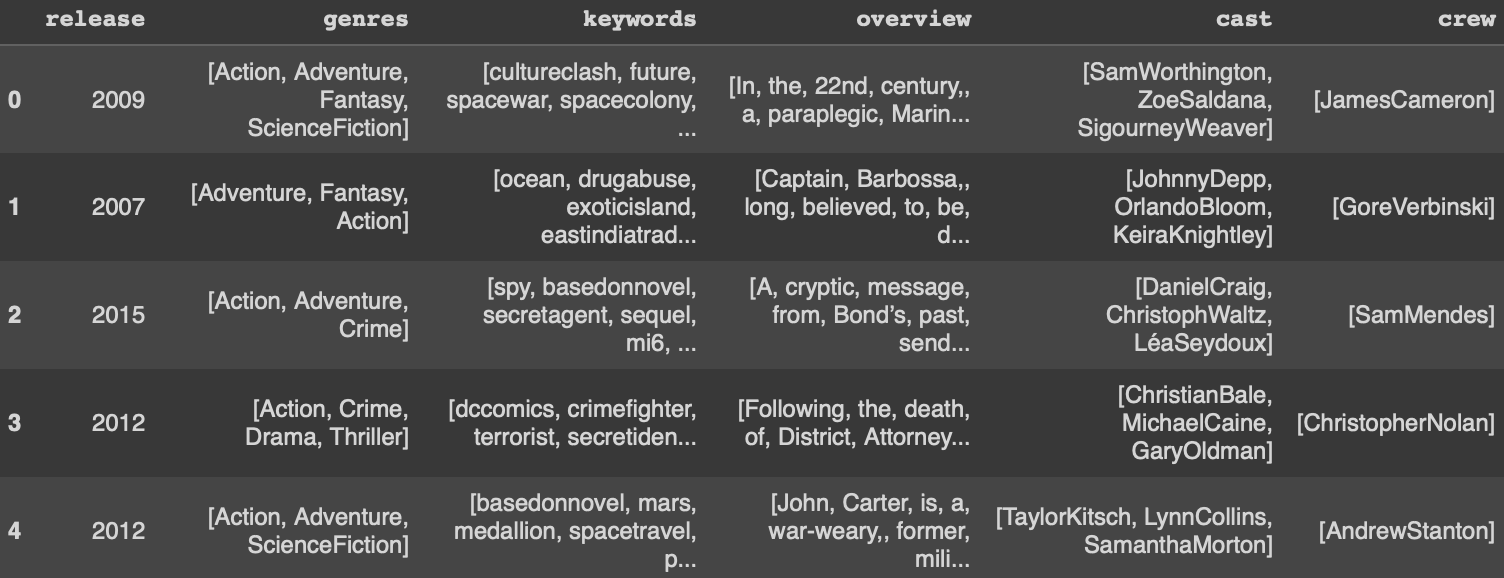
\includegraphics[width=1\linewidth]{screenshot/convert_featurefinal.png}
        \end{figure}
         
    \section{EDA: Analisi esplorativa del dataset}
        L’EDA è un approccio per analizzare ed esplorare i dati in modo da riassumere le caratteristiche principali del dataset.  In questo caso, è stata utilizzata l’EDA per comprendere meglio i dati a disposizione, e conseguentemente prendere decisioni su come costruire il sistema, come ad esempio quale modello di ML da utilizzare, come sviluppare la funzione di raccomandazione, quali filtri utilizzare ecc. Sono state esplorate le distribuzioni dei generi dei film, la popolarità dei film, le correlazioni tra le caratteristiche numeriche dei film, la distribuzione del budget dei film e i film con i maggiori incassi. Questo ha permesso di identificare nei dati quelli più affidabili, le tendenze, eventuali anomalie e i pattern, che hanno poi guidato lo sviluppo delle fasi successive del progetto. Di seguito verrano mostrati grafici derivanti dall'analisi esplorativa:
        \newpage
        \begin{figure}[H]
            \centering
            \begin{minipage}{.45\textwidth}
                \centering
                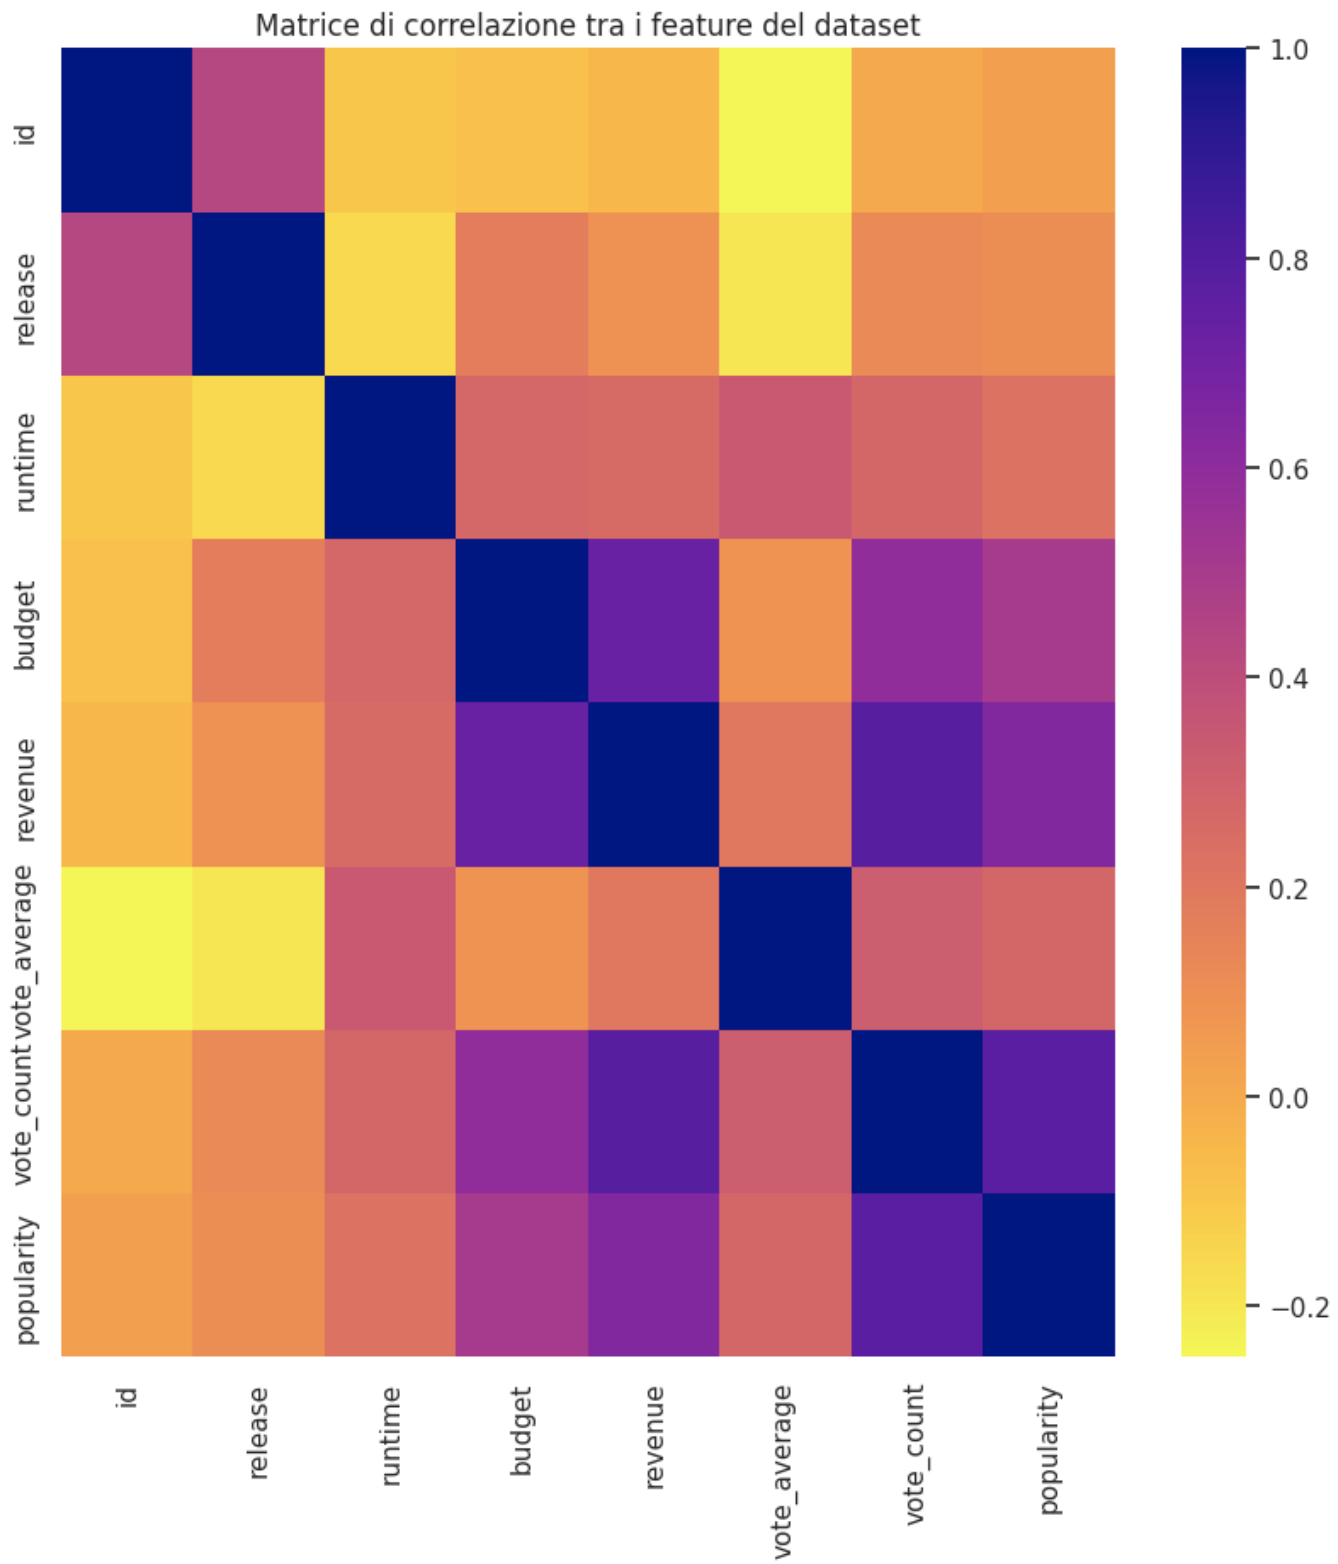
\includegraphics[width=1\linewidth]{EDA/eda3.png}
                \caption{Matrice di correlazioni tra le features numeriche}
                \label{fig:enter-label}
            \end{minipage}
            \begin{minipage}{.45\textwidth}
                \centering
                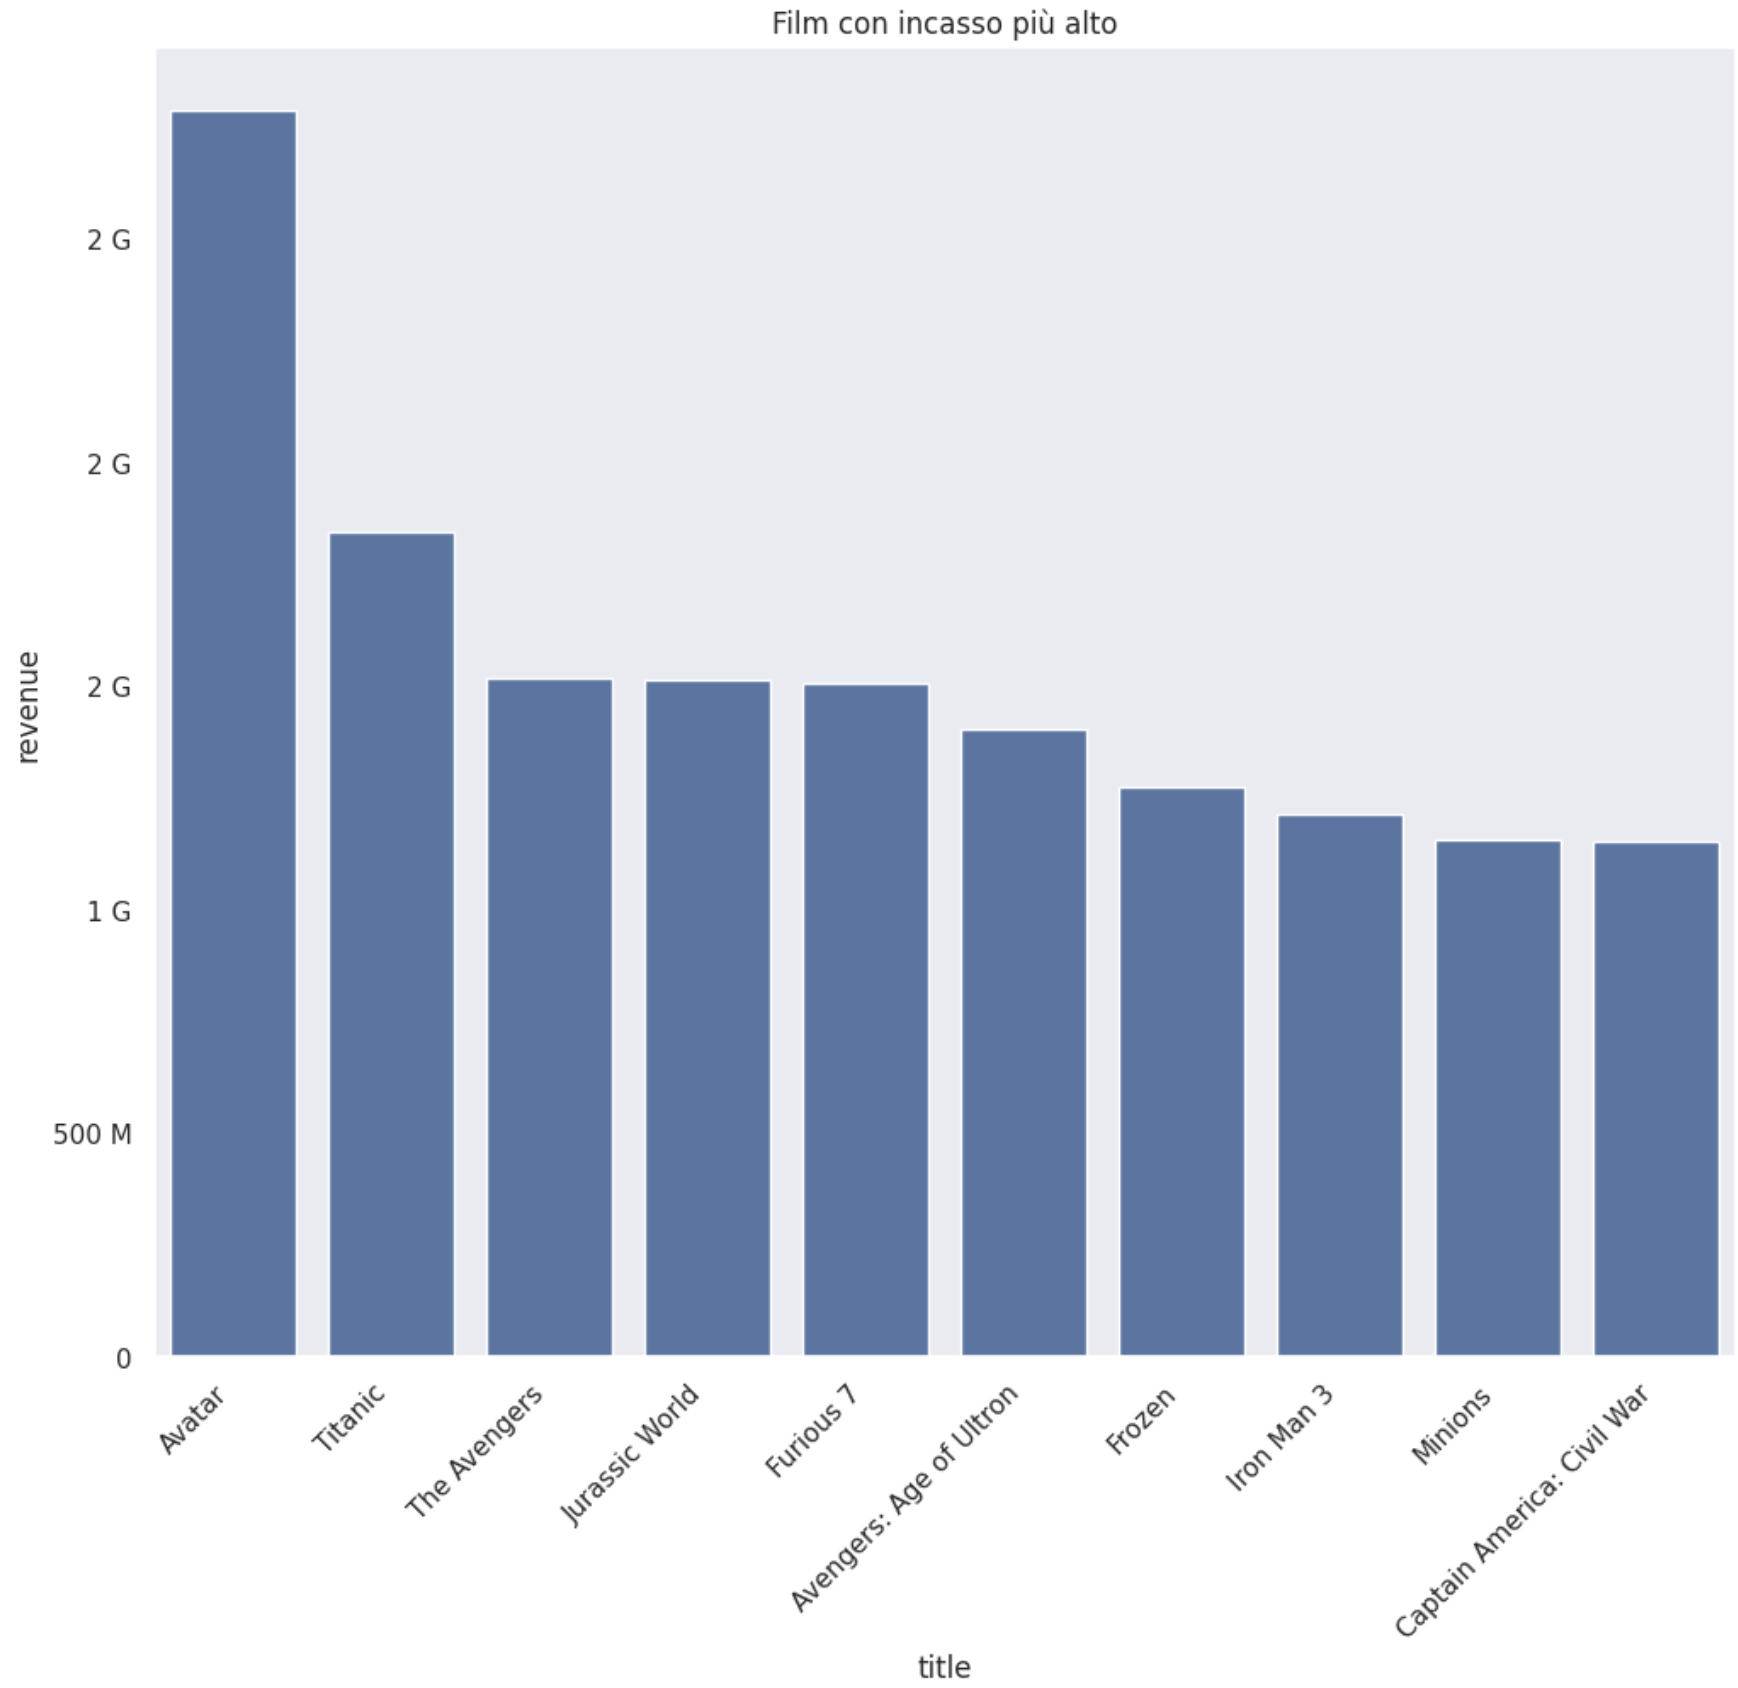
\includegraphics[width=1\linewidth]{EDA/eda6.png}
                \caption{Film con i ricavi più alti}
                \label{fig:enter-label}
            \end{minipage}
            \begin{minipage}{.45\textwidth}
                \centering
                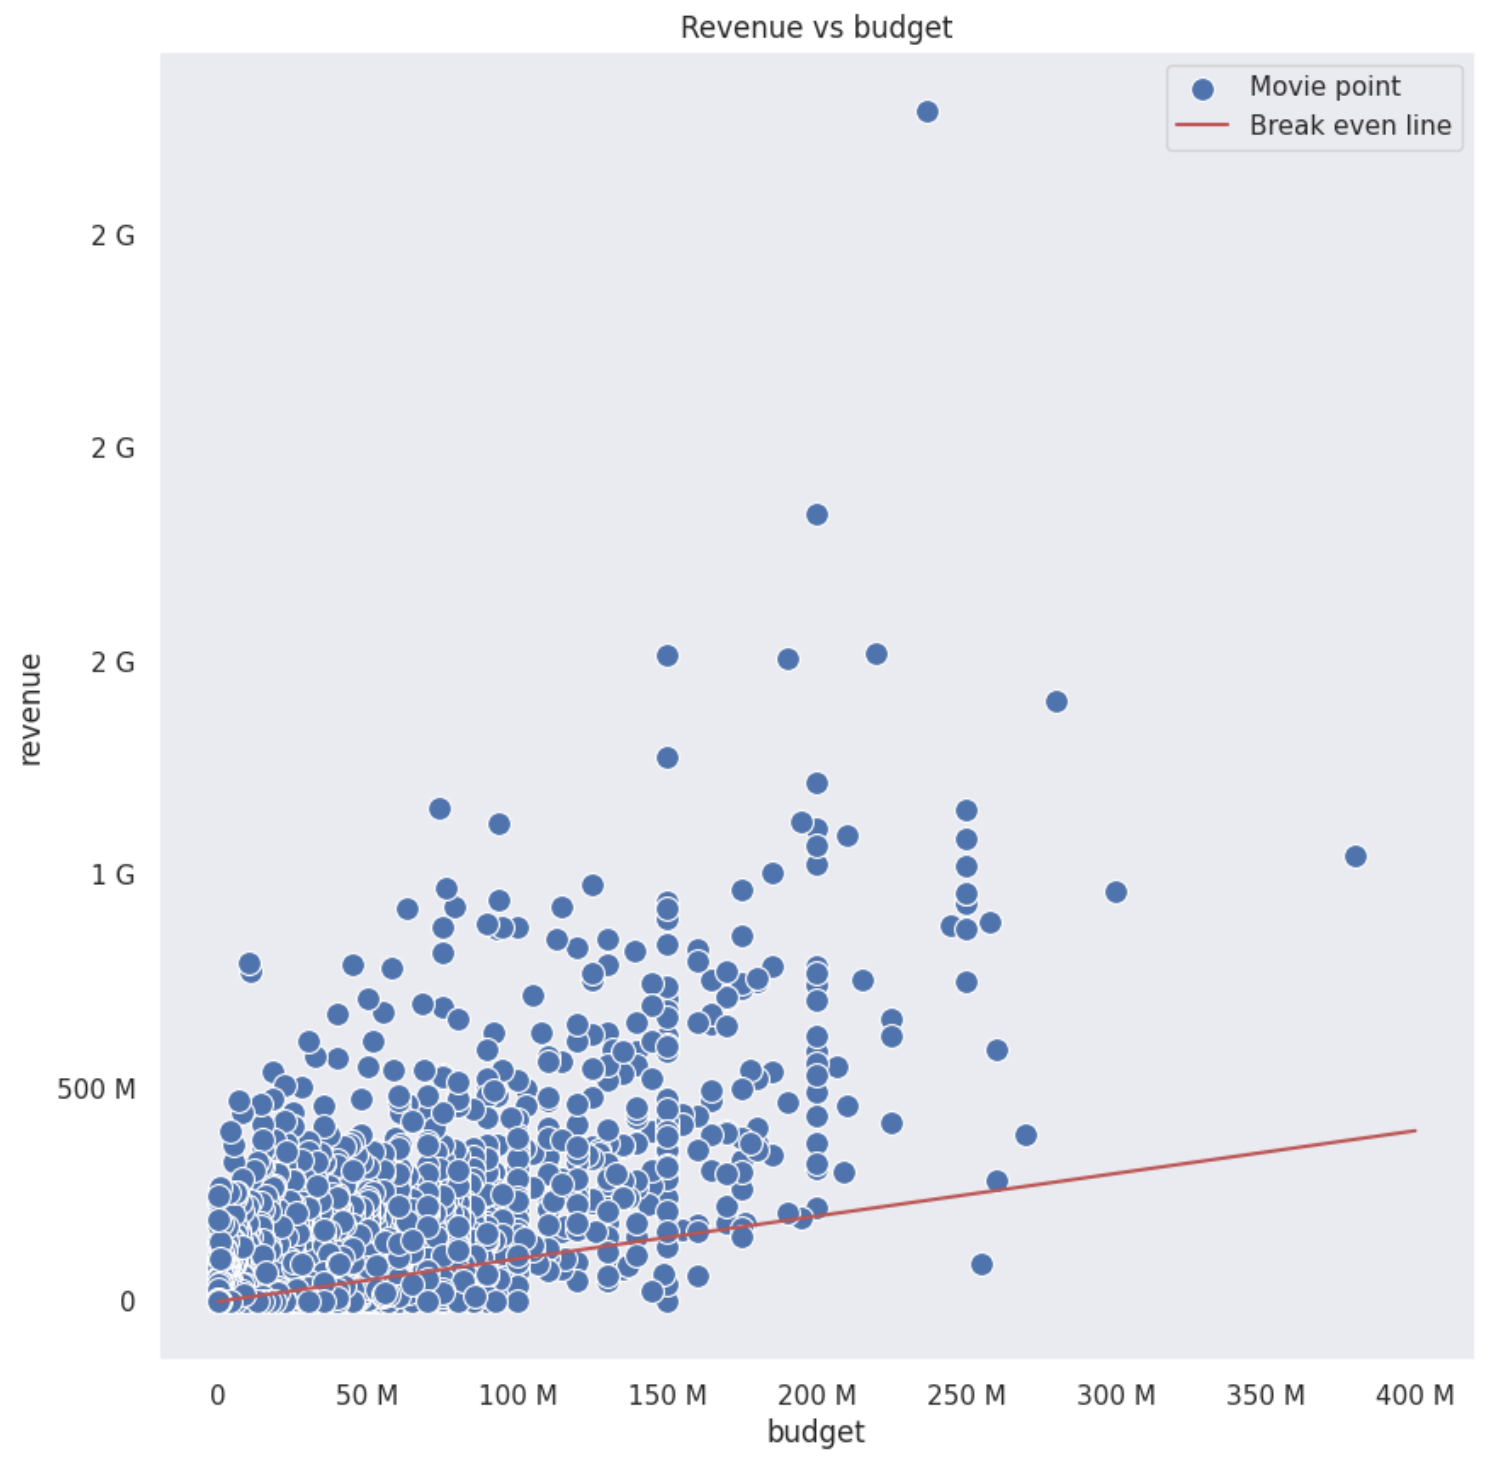
\includegraphics[width=1\linewidth]{EDA/eda5.png}
                \caption{Relazione tra il budget e il ricavo dei film}
                \label{fig:enter-label}
            \end{minipage}
            \begin{minipage}{.45\textwidth}
            \centering
            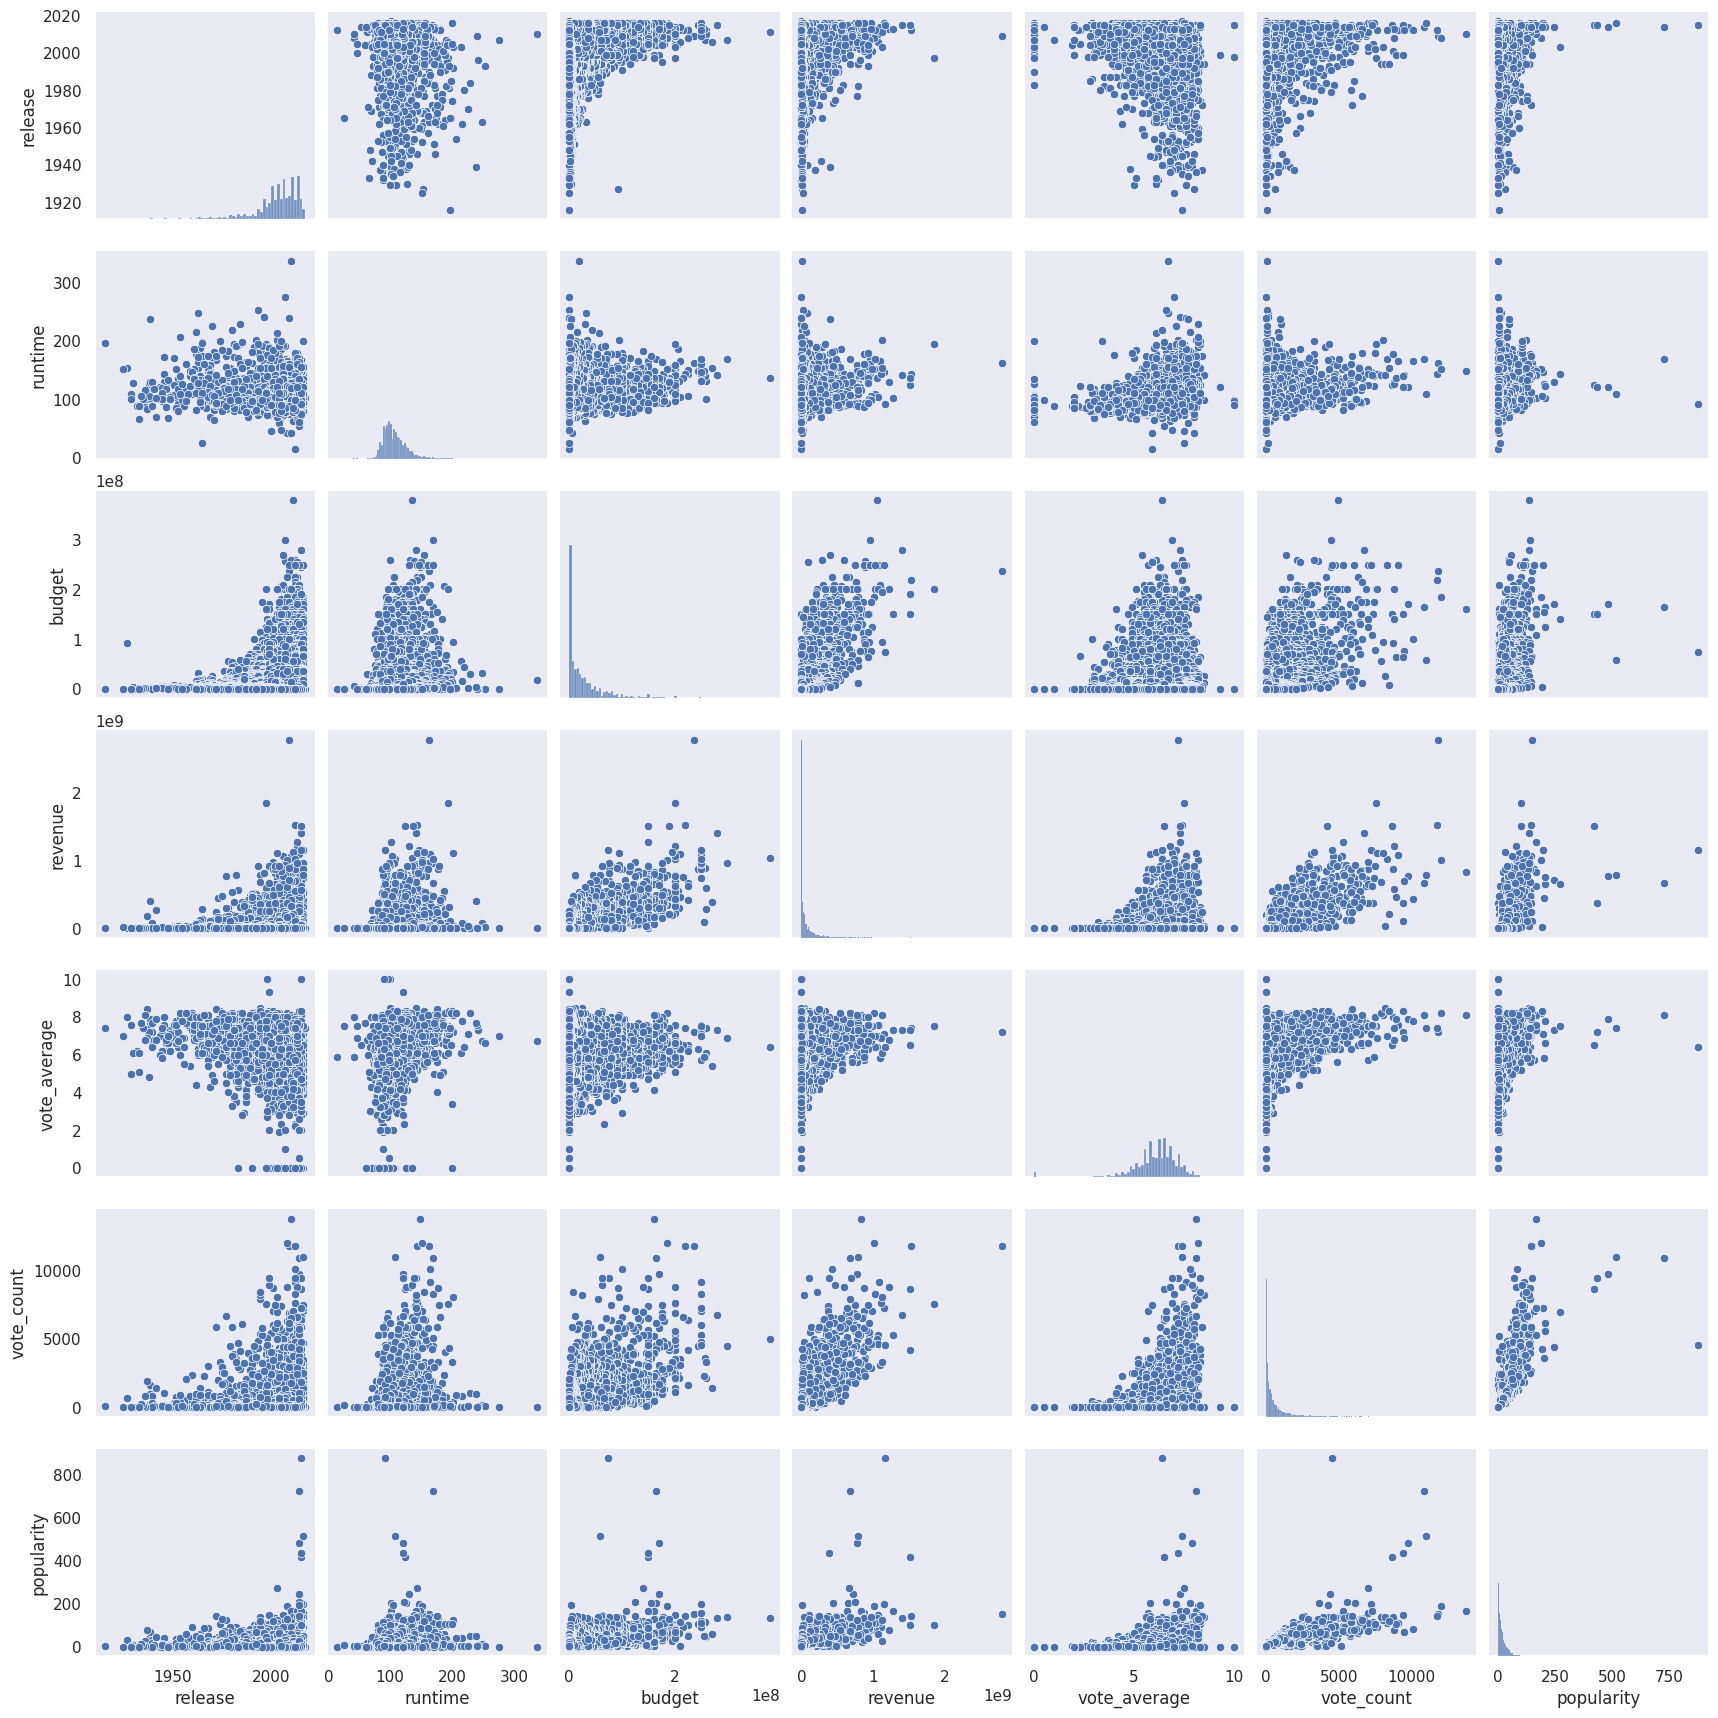
\includegraphics[width=1\linewidth]{EDA/eda7.png}
            \caption{Relazioni tra tutte le coppie di features numeriche}
            \label{fig:enter-label}
            \end{minipage}
            \begin{minipage}{.45\textwidth}
                \centering
                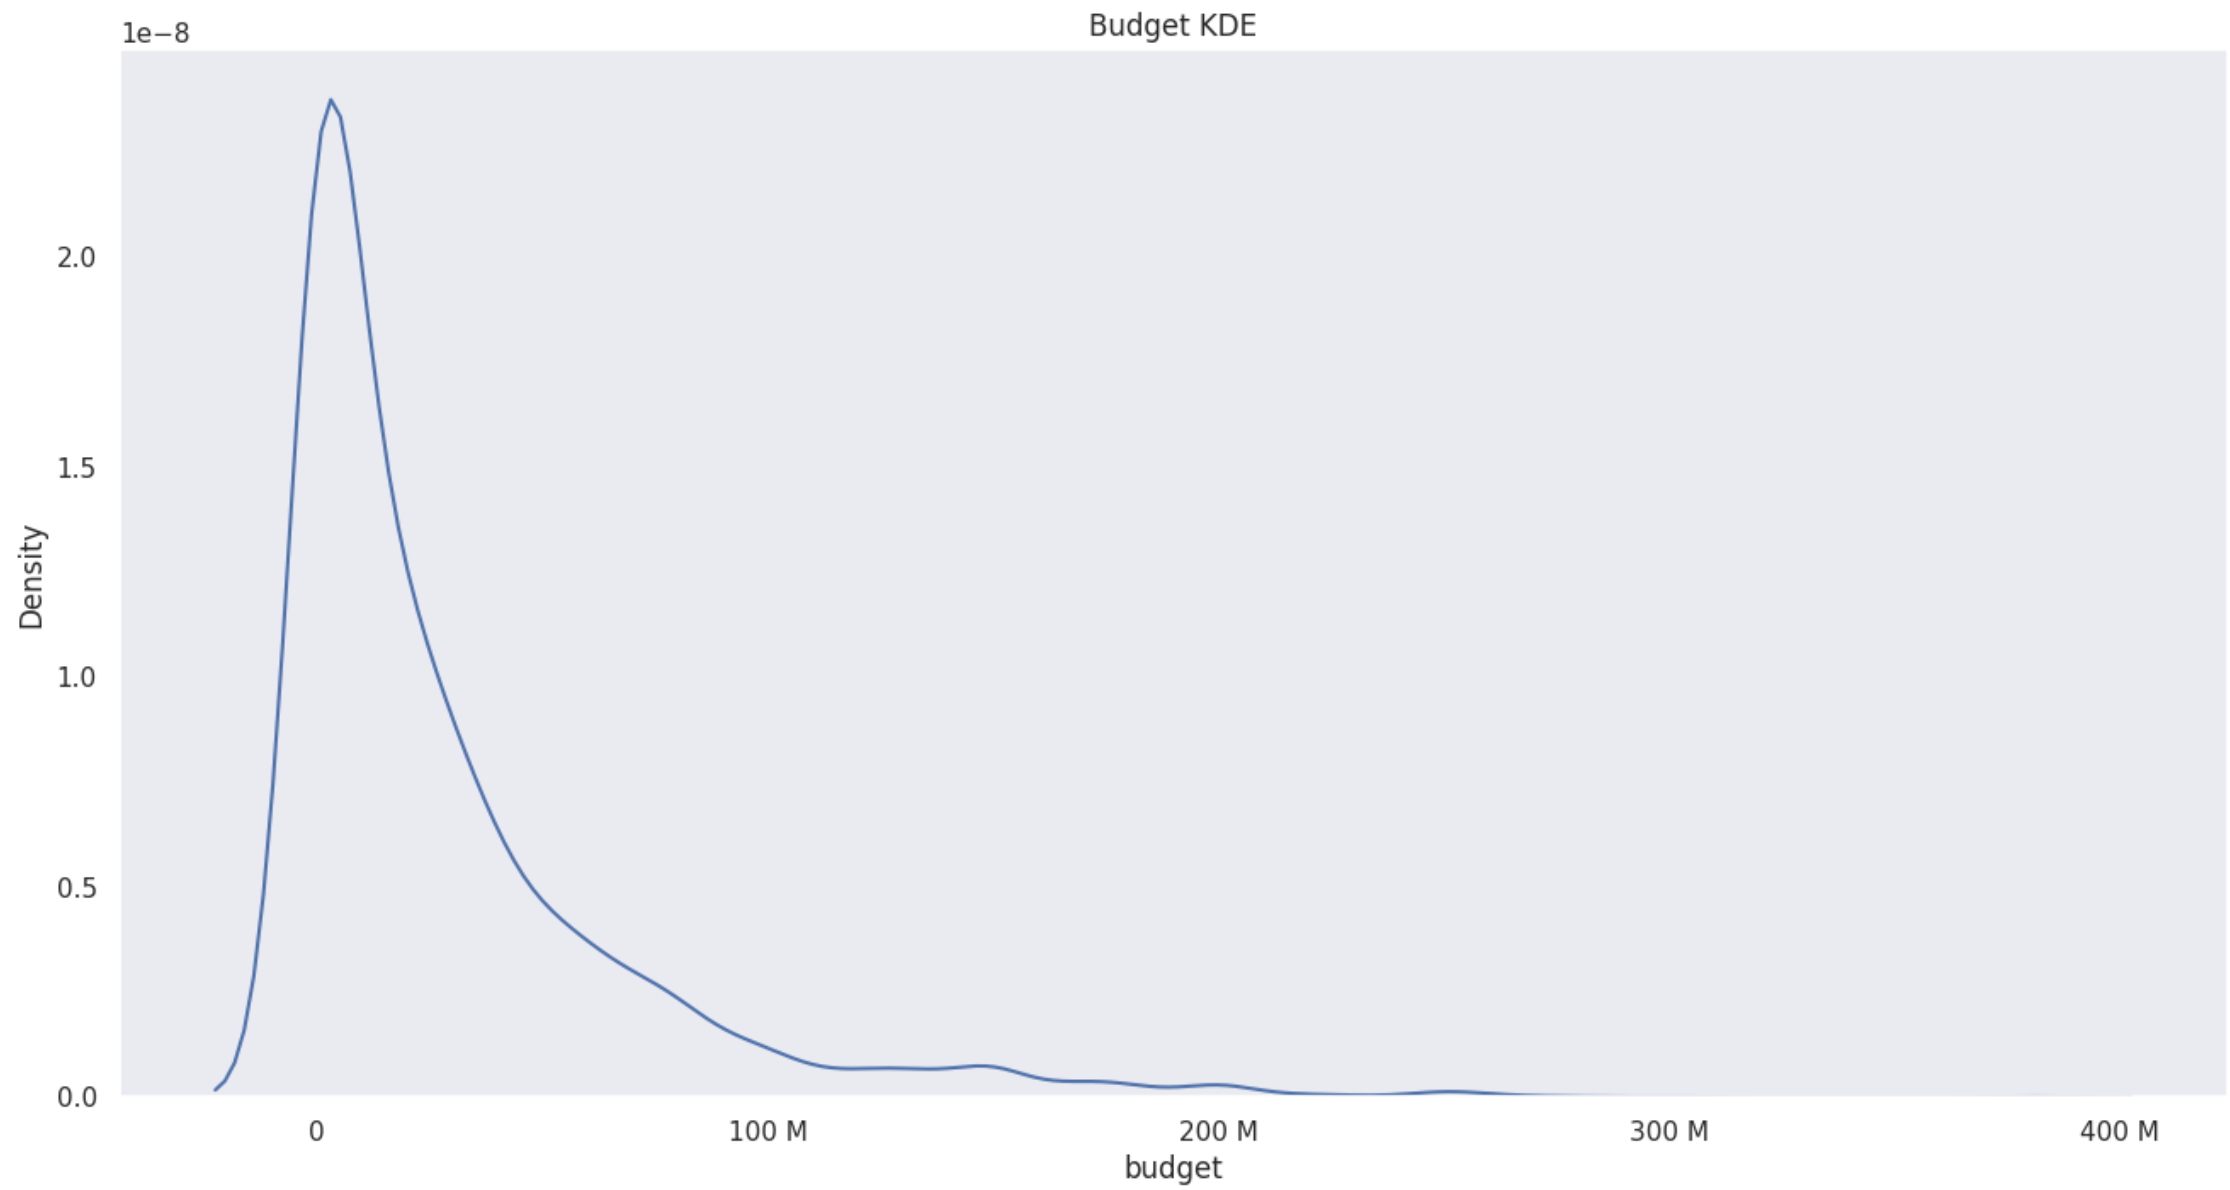
\includegraphics[width=1\linewidth]{EDA/eda4.png}
                \caption{Densità del kernel (KDE) della feature ‘budget’}
                \label{fig:enter-label}
            \end{minipage}
            \begin{minipage}{.45\textwidth}
                \centering
                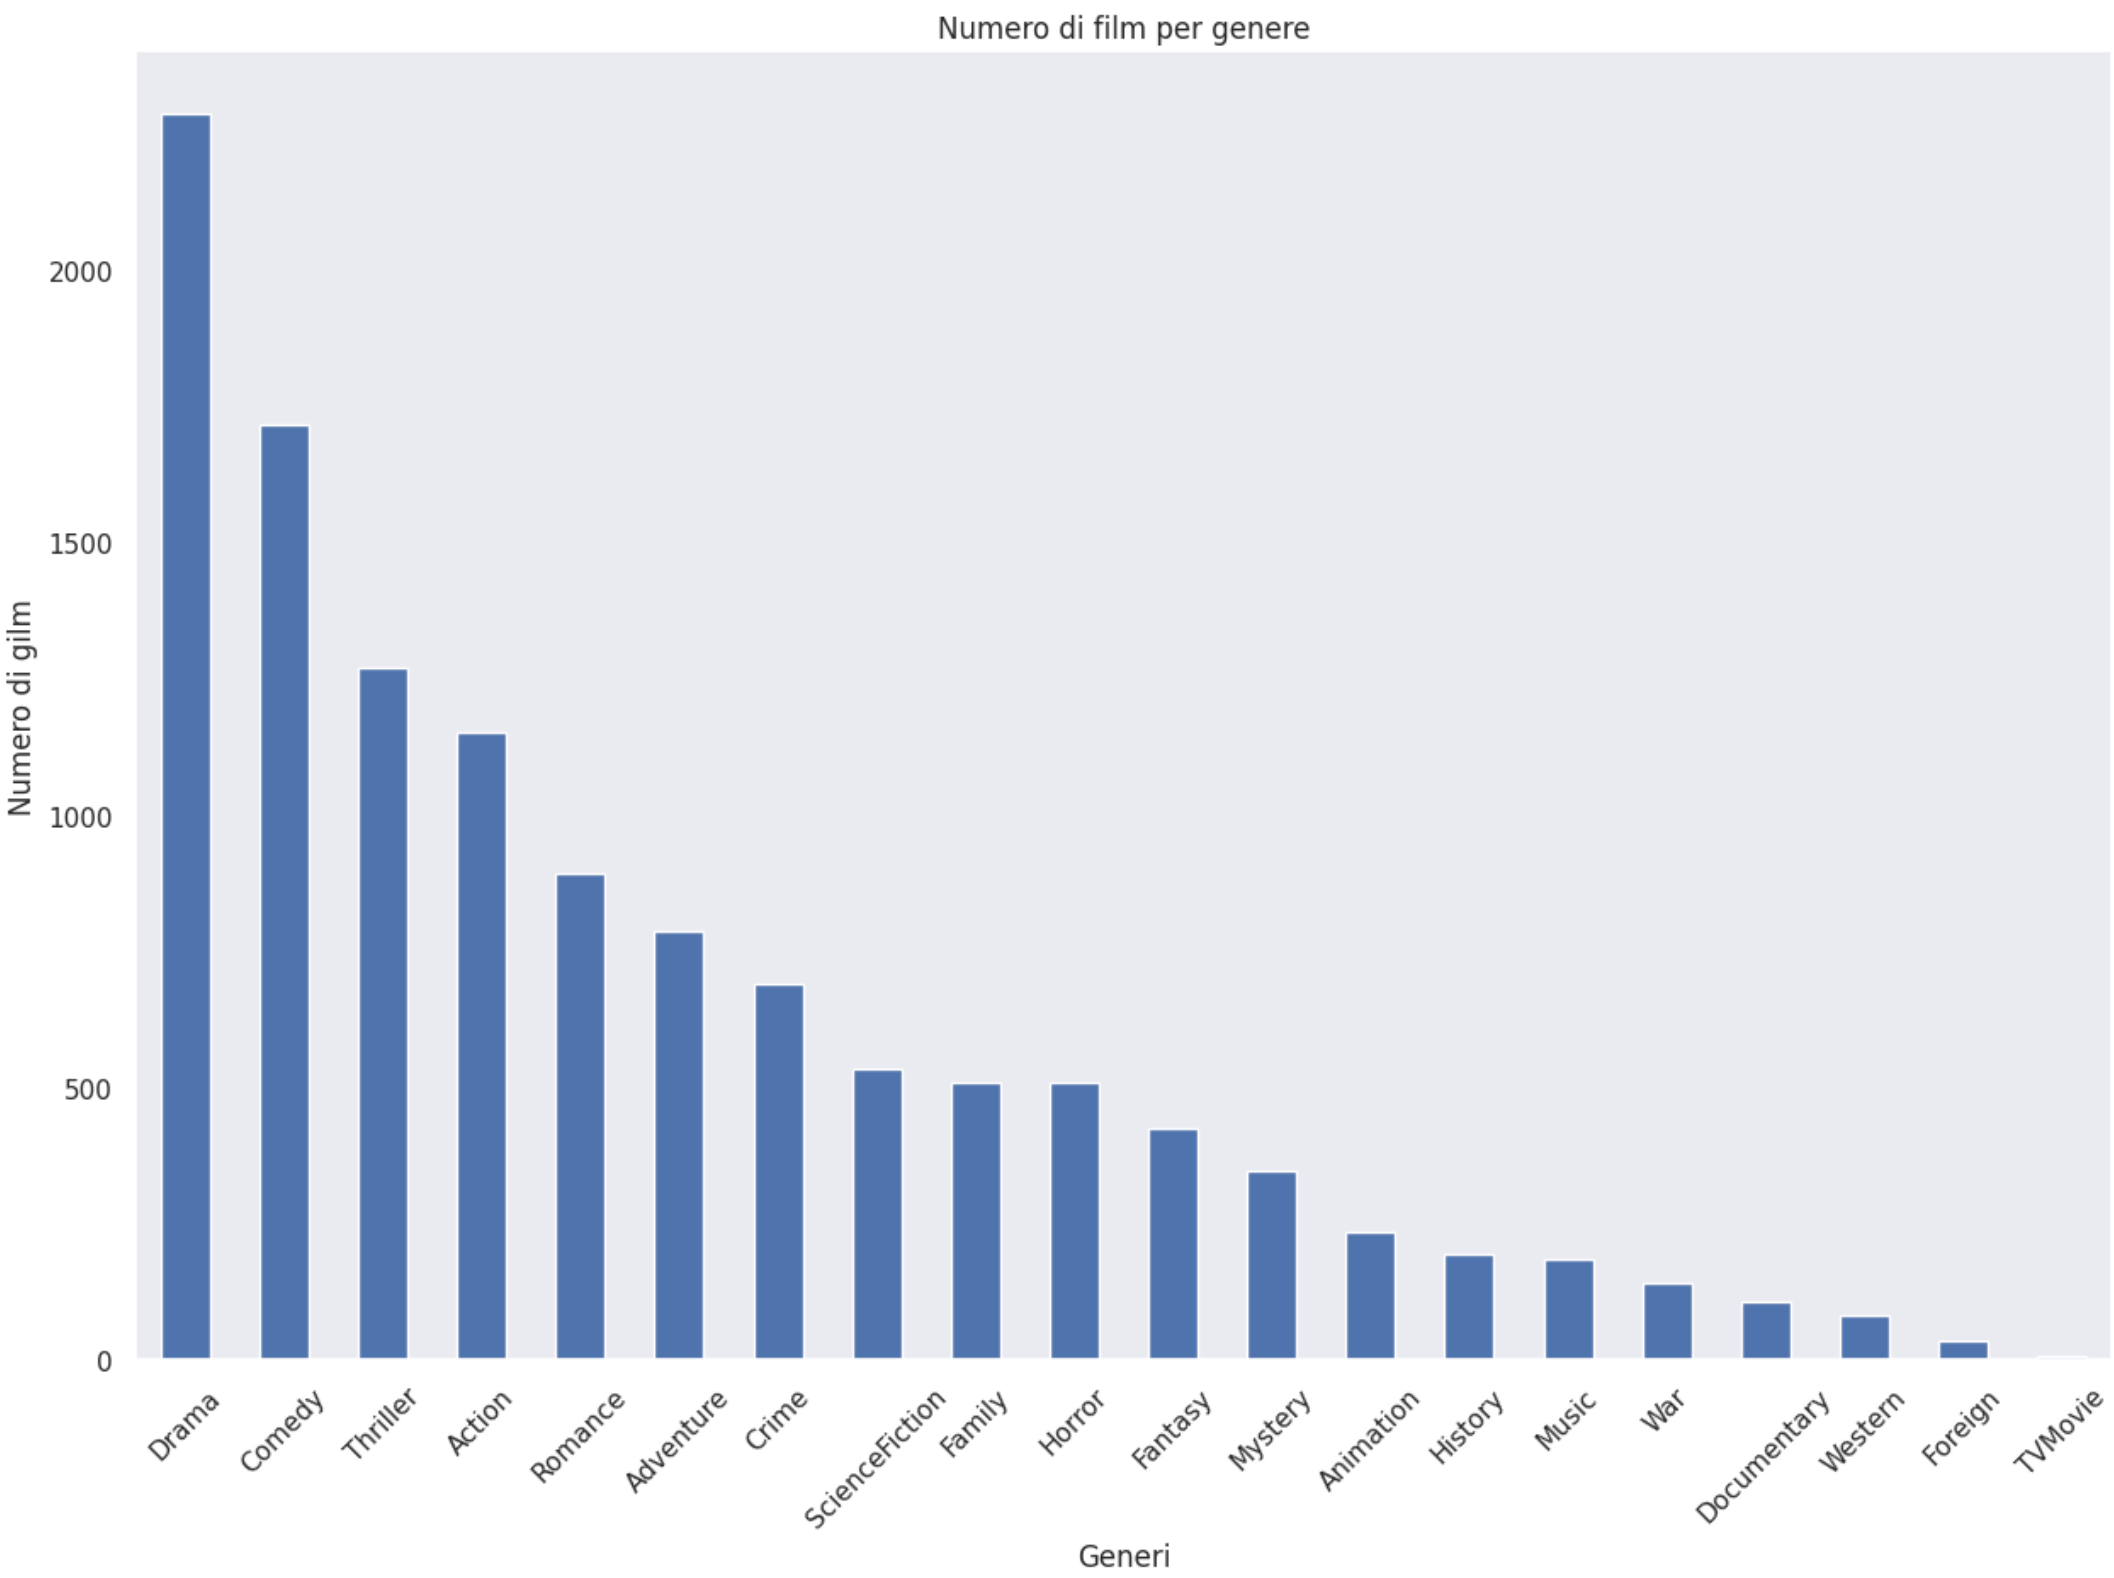
\includegraphics[width=1\linewidth]{EDA/eda2.png}
                \caption{Numero di film per ogni genere}
                \label{fig:enter-label}
            \end{minipage}
        \end{figure}
    \section{Machine Learning (ML)}
        Per la realizzazione del modello di Machine Learning viene utilizzato un Dataframe dedicato che presenta 3 features: id del film, nome del film, tags del film. Quest'ultima, ottenuta concatenando le feature "overview", "genres", "keywords", "cast", e "crew", è la feature chiave su cui si basa il funzionamento del modello, in quanto effettuerà raccomandazioni sui film in base a queste informazioni. Avendo concatenato diverse liste, difficili da gestire in questo caso, il campo tags viene trasformato in String e reso tutto in minuscolo, al fine di migliorare l'accuratezza delle raccomandazioni da parte del modello. \\
        Innanzitutto viene effettuata la feature extraction con CountVectorizer, una classe della libreria scikit-learn che trasforma il testo che riceve in input in una matrice numerica di conteggi di parole o token. Nel nostro caso è utile per ottenere dai dati grezzi un insieme di caratteristiche che verranno utilizzate per addestrare il modello. Al fine di facilitare il processo di riconoscimento di parole diverse ma correlate, viene applicata una funzione sulla feature tags che, attraverso l'algoritmo di Stemming di Porter (PorterStemmer) presente nella libreria NTLK, rimuove i suffissi comuni delle parole riducendole alla radice. Ciò viene fatto inoltre per ridurre la dimensione del vocabolario su cui il modello si baserà.\\
        La metrica utilizzata da parte del modello per effettuare raccomandazioni è quello della similarità del coseno. Nel Machine Learning, in particolare nei modelli che si basano su filtraggio del contenuto, la similarità del coseno viene utilizzata per determinare quanto sono simili due vettori (calcolati nel nostro caso con CountVectorizer) indipendentemente dalla loro dimensione. Infatti, questa metrica è particolarmente utile nel confronto di testi, nell’estrazione di dati e nell’analisi testuale. Matematicamente parlando, la similarità del coseno misura il coseno dell’angolo tra due vettori proiettati in uno spazio multidimensionale. Più è piccolo l'angolo di distanza, maggiore è la loro similarità. La similarità del coseno tra due vettori A e B viene calcolata come segue:
        \[ \text{{similarity}} = \cos(\theta) = \frac{{A \cdot B}}{{||A|| ||B||}} \]
        Dove:
        \begin{itemize}
            \item $A \cdot B$ è il prodotto scalare di A e B
            \item $||A||$ e $||B||$ sono le lunghezze (o norme) di A e B.
        \end{itemize}
        Attraverso questa metrica, viene quindi realizzata una matrice di similarità, che stabilisce quanto un film sia simile ad un altro in una scala che varia da 0 (meno simile) a 1 (più simile). \\
        Detto questo, può essere spiegata la funzione di raccomandazione, il fulcro del sistema: \\
        Quest'ultima prende in input un titolo di un film su cui si vuole riceve raccomandazioni ed eventuali filtri che si vogliono applicare: nel nostro caso si può filtrare per genere o insieme di generi, data di uscita, e/o durata del film.
        Nella prima parte di funzione, si esegue il modello di Machine Learning per ottenere i film più simili a quello dato in input. In caso non viene applicato alcun filtro, verrano direttamente restituiti i primi 5 film più simili (escluso il primo della lista perchè avrà indicatore di somiglianza 1, ovvero lo stesso film).      
        
    \section{Constraint Satisfaction Problem (CSP)}
        Applicando anche un solo filtro, ci sarà bisogno di creare un problema CSP, aggiungere le relative variabili e vincoli, risolverlo, e restituire le soluzioni.
        Infatti, la seconda parte di funzione prende in input i valori forniti dall'output del Machine Learning, per creare e risolvere un problema di soddisfazione dei vincoli (CSP). \\Calcolare le soluzioni di un problema creando variabili per ogni film presente nell'intero dataframe (circa 4800), richiederebbe un tempo di computazione elevato (nel nostro caso più di 30 secondi). Prendendo in input i risultati del ML invece, dove è stato scelto di restituire i 1000 film più simili per garantire un margine di ricerca, il tempo di computazione viene ridotto a pochi secondi. L'obiettivo della risoluzione del Constraint Satisfaction Problem è quello di restituire un insieme di film che soddisfano determinati vincoli (genere, anno di uscita, durata) al fine di realizzare un filtro dei risultati.
        Quindi, inizialmente viene creato un problema CSP in cui ogni film è una variabile con dominio [True, False]. 
        \begin{itemize}
            \item \textbf{True} se il film è selezionato
            \item \textbf{False} se il film non è selezionato
        \end{itemize}
        Dopo aver aggiunto le variabili per ogni film raccomandato dal ML, vengono aggiunti i vincoli in base alla scelta da parte dell'utente dei criteri di "genere", "anno di uscita" e "durata".
        Infine, viene risolto il problema CSP per trovare tutte le soluzioni che soddisfano i vincoli, da cui si ricavano i film selezionati; questi ultimi sono l'elenco di film che rispettano i filtri applicati, e che possono essere raccomandati. \\
        Le soluzioni CSP sono ordinate in ordine alfabetico di default. Nel nostro caso non va bene perchè vogliamo restituire le prime 5 soluzioni, e potrebbe non essere una soluzione ottimale. Per questo, è stato pensato di ordinare le soluzioni per votazioni da parte degli utenti; in particolare per avere un dato attendibile, perchè ad esempio potrebbero esserci film con media voto 10 con due sole votazioni, viene calcolata la feature "score" su cui eseguire l'ordinamento delle soluzioni. Si procede quindi a costituire la formula di ponderazione del voto medio, la stessa metrica utilizzata ad esempio da IMDb, che tiene conto sia del voto medio del film che del numero di voti ricevuto. Segue la seguente la formula matematica:
        \[ \text{{score}} = \frac{{\text{{vote\_count}}}}{{\text{{vote\_count}} + m}} \cdot \text{{vote\_average}} + \frac{{m}}{{\text{{vote\_count}} + m}} \cdot c \]
        Dove:
        \begin{itemize}
            \item $c$ è la media di tutte le medie dei voti dei film
            \item $m$ è il minimo numero di voti richiesti affinché il film sia elencato. In questo caso m è calcolato come il quantile 0.9 del conteggio dei voti di tutti i film. In altre parole, m è il valore sotto il quale cade il 90\% dei conteggi dei voti.
        \end{itemize}
        Quindi saranno restituiti all'utente i primi 5 film ordinati per punteggio all'interno delle soluzioni del problema CSP. 
        
    \section{Interfaccia grafica}
        \begin{figure}[h]
            \centering
            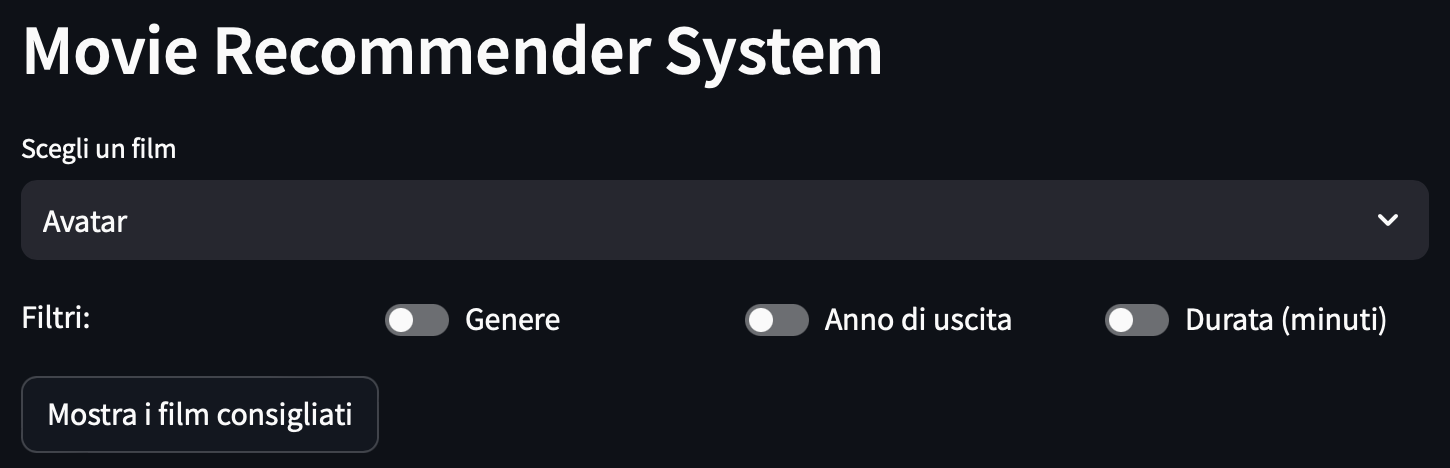
\includegraphics[width=1\linewidth]{screenshot/sezioni_1.png}
        \end{figure}
        Per far sì che l'utente possa interagire con il sistema è stata realizzata un applicazione web che funge da interfaccia grafica utilizzando la libreria python "Streamlit", un framework open source che consente di creare applicazioni ottimizzate per l'uso del Machine Learning.
        L'interfaccia presenta diverse sezioni, la prima è quella dove possiamo ottenere raccomandazioni da parte del sistema:
        inserendo il film desiderato e cliccando su "Mostra Risultati", sul lato back-end viene richiama la funzione di raccomandazione dichiarata nel codice sorgente principale per processare i risultati (viene quindi effettuato il riutilizzo del codice), e sul lato front-end mostra i film raccomandati, dove per ogni film verrà mostrato:
        \begin{itemize}
            \item \textbf{Titolo} del film
            \item \textbf{Copertina}: interagendo con l'API di TMDb si ottengono i poster dei film in realtime direttamente da TMDb
            \item \textbf{Info}: un link che riporta alla homepage del film sul sito di TMDb. Questo verrà calcolato dinamicamente per ogni film tramite la funzione "movie\_link" che andrà a concatenare oppurtunamente l'URL
        \end{itemize} 
        
        Ispirandosi ai diversi recommender system quali ad esempio quelli di Amazon, Netflix o Spotify, sono state riportate altre sezioni che indicano rispettivamente i film più visti al cinema, i film più popolari, e le nuove uscite. Ciò è stato fatto non solo per rendere l'interfaccia completa, ma anche per migliorare la user experience fornendo raccomandazioni aggiuntive.
        \begin{figure}[h]
            \centering
            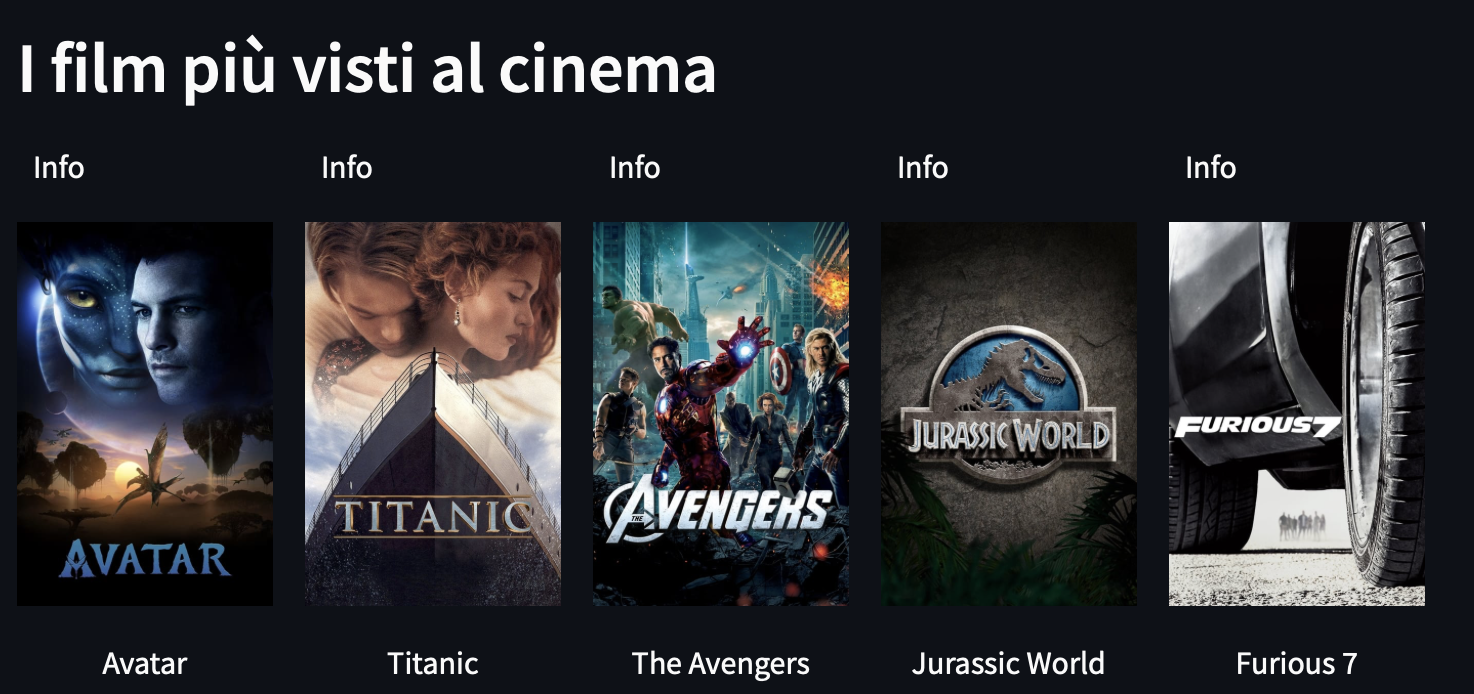
\includegraphics[width=1\linewidth]{screenshot/sezioni_2.png}
            \caption{(1/3) Sezione "Film più visti"}
            \label{fig:enter-label}
        \end{figure}
        \begin{figure}[h]
            \centering
            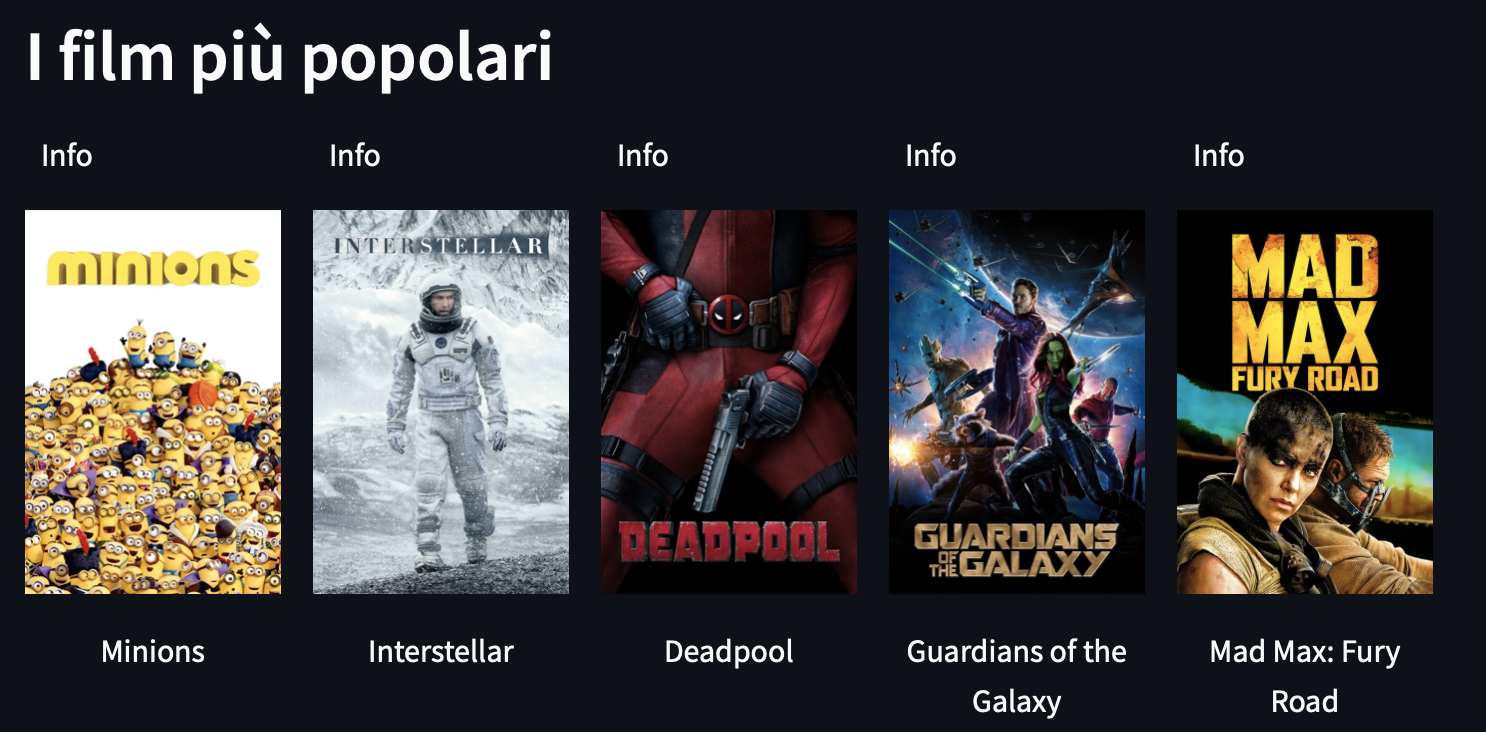
\includegraphics[width=1\linewidth]{screenshot/sezioni_3.png}
            \caption{(2/3) Sezione "Film più popolari"}
            \label{fig:enter-label}
        \end{figure}
        \begin{figure}[h]
            \centering
            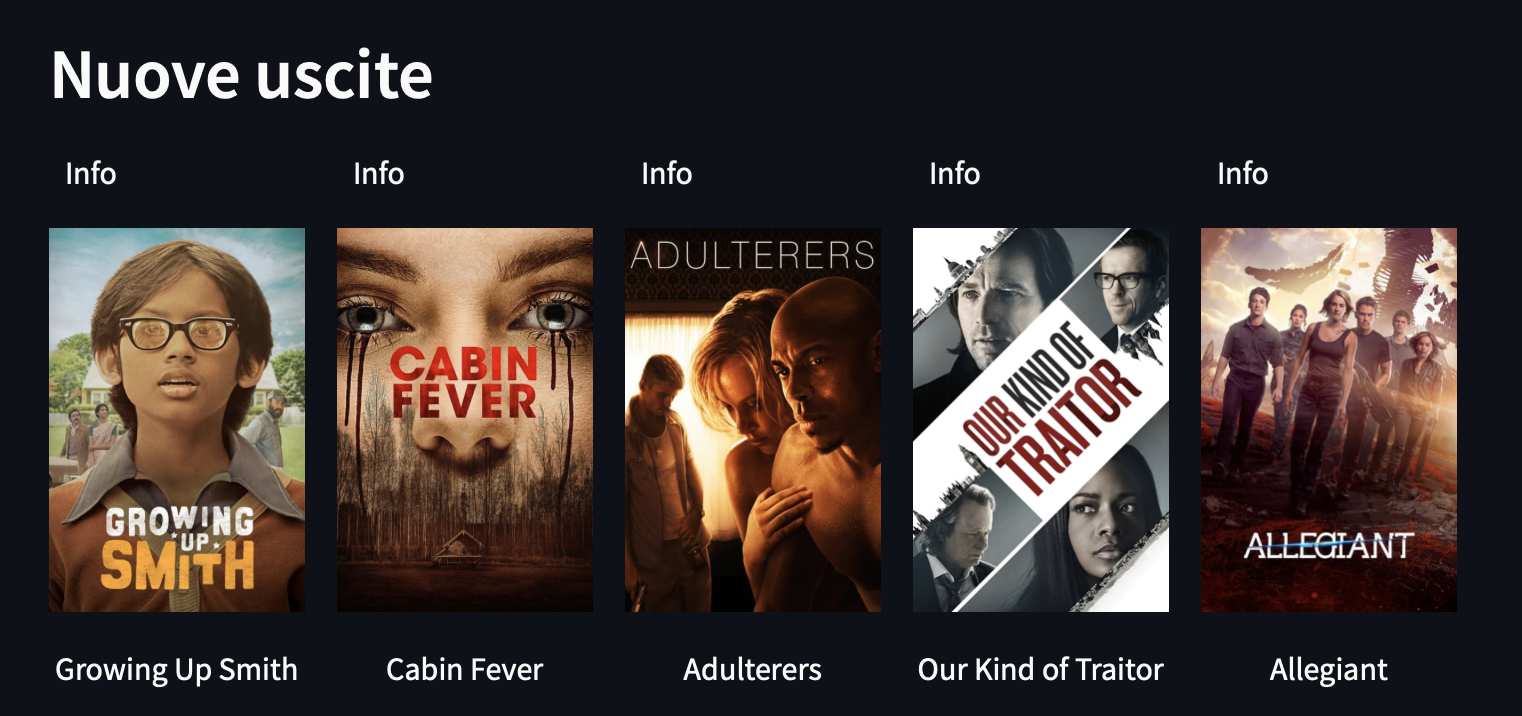
\includegraphics[width=1\linewidth]{screenshot/sezioni_4.png}
            \caption{(3/3) Sezione "Film più recenti"}
            \label{fig:enter-label}
        \end{figure}
        
\chapter{Esperimenti e Risultati}
    \section{Scelta del dataset}
        Per la realizzazione del recommender system è stato valutato di scegliere altri dataset, come ad esempio quello di "Movielens". Probabilmente con questa scelta si sarebbero potuti avere più film a disposizione. Tuttavia:
        \begin{enumerate}
            \item Il numero di dataset da includere sarebbe stato maggiore, e ognuno possedeva molti più dati
            \item Sarebbe aumentata la possibilità di avere dati inconsistenti/incompleti, e di conseguenza anche la fase di pulizia e preparazione del dataset sarebbe stata più "tortuosa"
            \item I tempi di computazione sarebbero aumentati
            \item Il recupero del poster del film da TMDb tramite API e dei link dei film non sarebbe stato immediato dato che il dataset non è lo stesso
        \end{enumerate}
        Di conseguenza, la scelta è caduta sul dataset di TMDb di Kaggle.com in quanto le features con i relativi dati e i tempi di computazione li abbiamo ritenuti validi e opportuni per il raggiungimento dell'obiettivo del nostro sistema, ovvero quello di effettuare raccomandazioni basate sul contenuto. Inoltre, il fatto che fosse di TMDb ha permesso la realizzazione di collegamenti diretti con il sito (API e link alla trama).
    \section{Scelta del modello di Machine Learning}
        Per la realizzazione della componente di Machine Learning sono stati valutati diversi approcci oltre quello scelto, in particolare è stato valutato di implementare un modello di \textbf{regressione lineare} o di \textbf{filtraggio collaborativo}. \\
        Nel primo caso, il modello è stato riscontrato essere non opportuno per l'obiettivo da raggiungere, in quanto viene utilizzato in particolare per la previsioni di valori ad esempio nel campo di Finance. Nel secondo caso, l'approccio di filtraggio collaborativo, che effettua quindi raccomandazioni basandosi su recensioni degli utenti, è stato riscontrato essere sicuramente più pertinente, e probabilmente con quest'ultimo si sarebbero potuti ottenere risultati interessanti. Tuttavia, avrebbe richiesto l'inclusione di un altro dataset di recensioni, cosa che avrebbe aumentato i tempi di computazione generali. La scelta è quindi stata quella di realizzare un modello che utilizza un approccio di filtraggio basato sul contenuto, pagando come "tradeoff" il fatto di avere probabilmente una precisione minore sulle raccomandazioni, ma tempi di computazione più veloci.
    \section{Inclusione ML + CSP}
        Nella funzione di raccomandazione, l'output della componente Machine Learning è l'input della componente CSP. È stato sperimentato l'inversione dei due componenti, ovvero output del CSP che diventa input del ML, ma è stato riscontrato un calo delle performance notevole e un aumento del tempo di esecuzione esponenziale. Infatti in questo modo, bisognerebbe calcolare le soluzioni del problema CSP di tutto il dataset, cosa che nel nostro caso ha richiesto più di 30 secondi. Includendo invece i componenti come specificato all'inizio, l'esecuzione della funzione di raccomandazione si riduce a pochi secondi.
    \section{Generazione dei risultati}
        \begin{figure}[h]
            \centering
            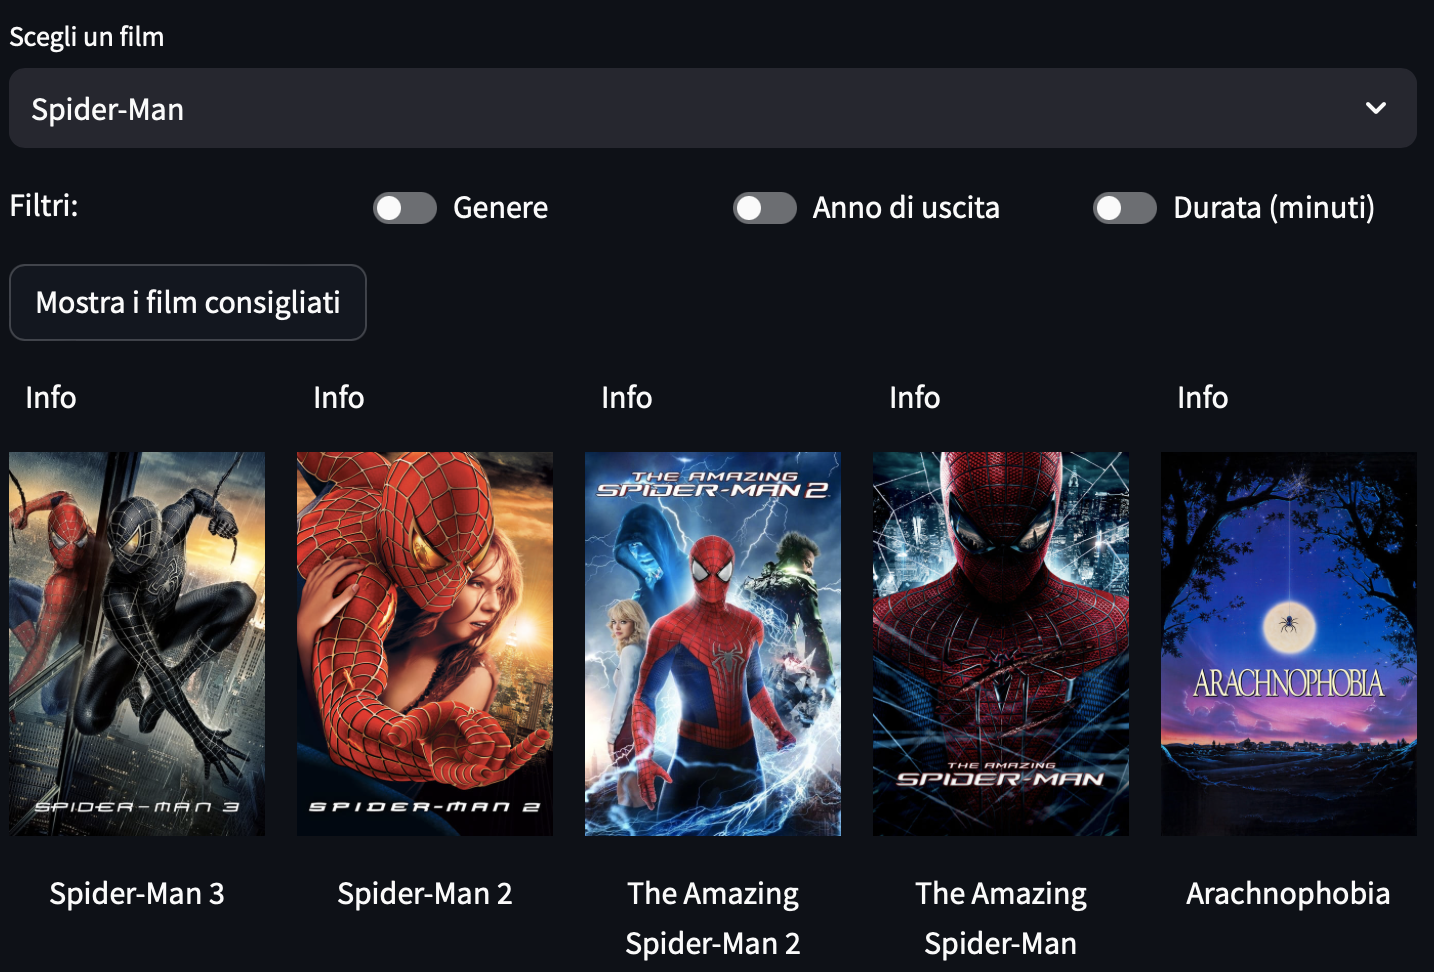
\includegraphics[width=1\linewidth]{screenshot/ricerca_nofilters.png}
        \end{figure}
        Come menzionato nel capitolo precedente, se l'utente sceglie di non selezionare alcun filtro di ricerca, verranno restituiti semplicemente i film più simili a quello richiesto. 
        In caso si decidesse di filtrare, basta premere uno o più toggle desiderati, selezionare i relativi valori, e mostrare i risultati.
        \begin{figure}[h]
            \centering
            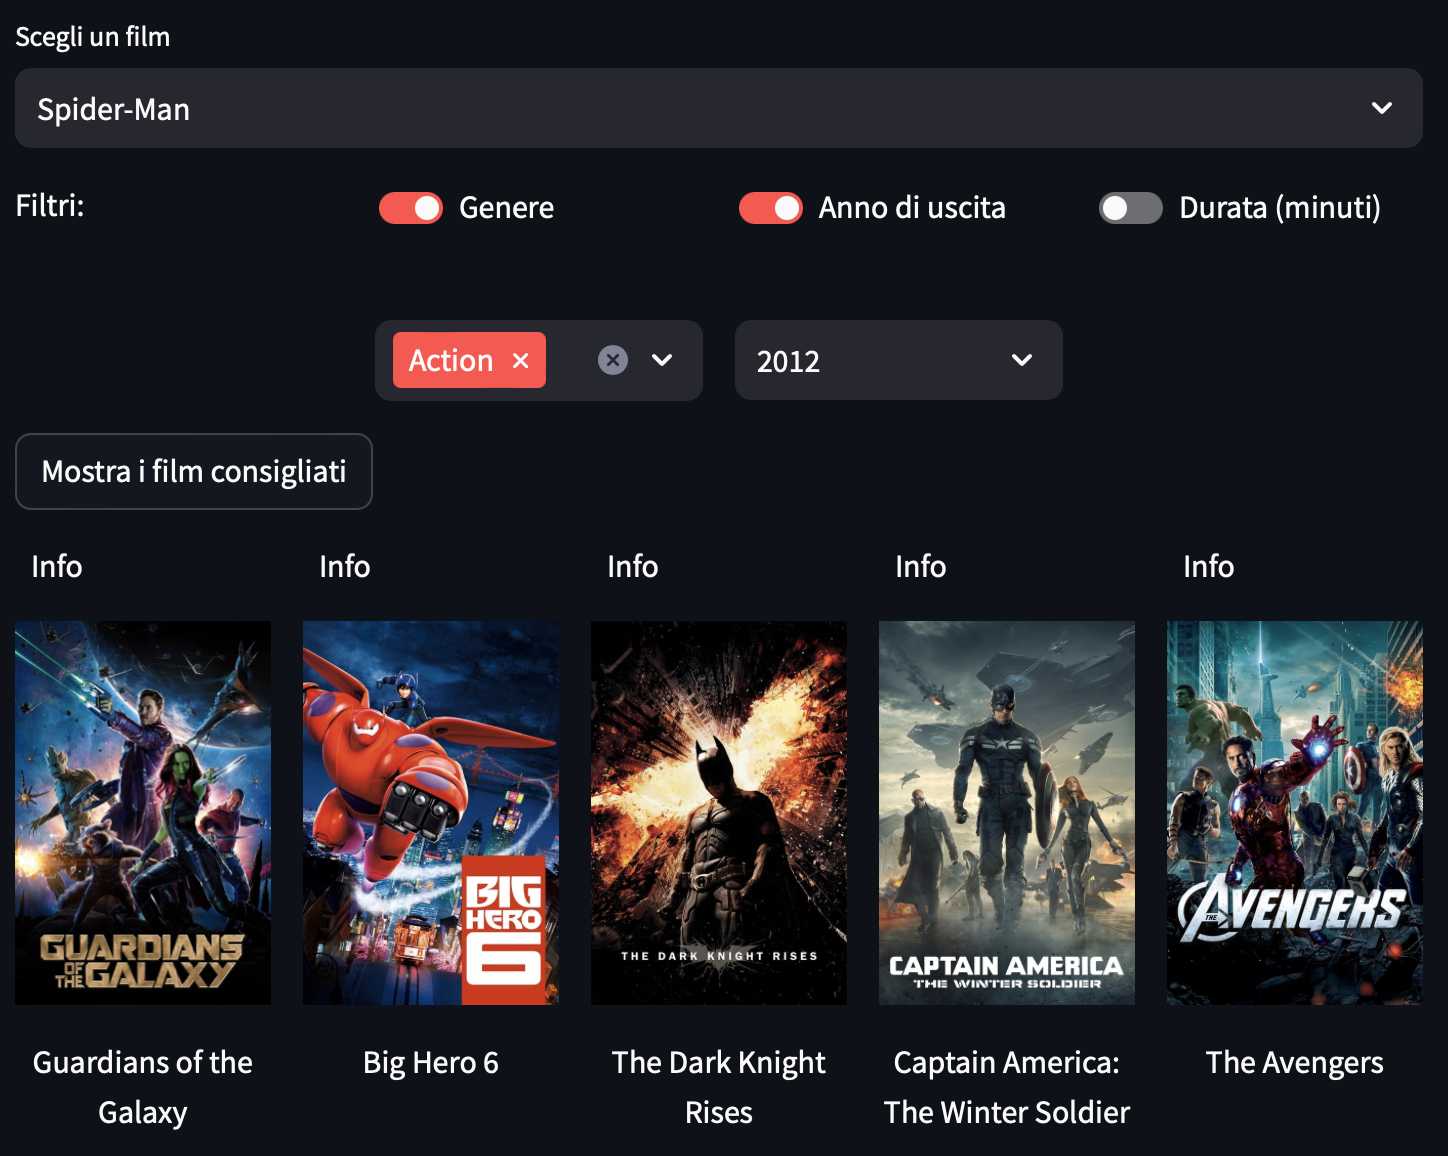
\includegraphics[width=1\linewidth]{screenshot/ricerca_filters.png}
        \end{figure}
        \\Le raccomandazioni variano notevolmente a seconda dei vincoli forniti dall’utente. Ad esempio, se un utente richiede che i film da raccomandare siano di un certo genere, verranno restituiti film che avranno quel genere. Aggiungendo un altro genere, verranno raccomandati film che contengono entrambi i generi. Allo stesso modo, aggiungendo filtri come l'anno di uscita o con una certa durata, la lista di film raccomandati sarà più ristretta.

\chapter{Conclusioni}
Giunti alle conclusioni, il sistema rispecchia totalmente l'obiettivo che abbiamo prefissato di raggiungere: costruire un recommender system di film con approccio di filtraggio basato sul contenuto. Il sistema è semplice, intuitivo, fornisce risultati attendibili, e risponde con tempi di esecuzione convincenti. \\
La sua scalabilità suggerisce inoltre possibili lavori futuri che potrebbero essere svolti in merito. La struttura permette infatti non solo di essere applicata ad altri ambienti come e-commerce o streaming di contenuti, ma anche di ampliarlo ad esempio raccomandando più film, inserendo più filtri, o inserendo più sezioni nella homepage dell'interfaccia grafica. 
Un altro suggerimento per lo sviluppo di questo sistema potrebbe essere quella di adottare un approccio ibrido di Machine Learning, che combina tecniche di apprendimento supervisionato e non supervisionato: un esempio interessante potrebbe essere quello di utilizzare un approccio ibrido tra filtraggio basato sul contenuto e filtraggio collaborativo, al fine di migliorare la precisione e l'attendibilità delle raccomandazioni dei film.
\end{document}
